\section{Runterschreiben}
\label{sec:rusch}



\subsection{Entwicklung des Agentenplanes + \enquote{Tuning}}

Die mathematischen Gleichungen in \cite{na-sch} beschreiben gut, welches Verhalten dem Agenten zu geben ist: wenn möglich beschleunigen, zufällige Reduktion der Geschwindigkeit (Trödeln) und wenn nötig abbremsen.

\subsubsection{Zustandsautomat}

Das Verhalten wurde mit einem endlichen Automaten beschrieben, siehe [Grafik Automat].
[GRAFIK]

Startzustand ist ein allgemeiner Zustand \enquote{Fahren} (DRI), in dem nichts am Verhalten des Agenten geändert wird.
Von hier aus ist der Zustand \enquote{Beschleunigen} (ACC) zu erreichen, wenn die aktuelle Geschwindigkeit unter der max. zulässigen liegt. 
Der Zustand \enquote{Cruisen} (CRU) wird erreicht, wenn die max. zulässige Geschwindigkeit überschritten ist.

Die Übergänge aus den zwei letztgenannten Zuständen sind identisch. 
Ist kein vorausfahrender Verkehr vorhanden und wird nicht getrödelt erfolgt der Übergang zurück in den normalen DRI-Zustand.
Wir stattdessen zufällig das \enquote{Trödeln} angestoßen wir der entsprechende Zustand (LIN) erreicht.
Ist Verkehr voraus wird der Zustand enquote{Verzögern/Bremsen} (DEC) erreicht.

Aus dem DEC-Zustand kann zufällig ein Übergang in den LIN-Zustand erfolgen ansonsten zurück in den allgemeinen DRI-Zustand.
Aus dem LIN-Zustand wird zwangsläufig wieder in den DRI-Zustand übergegangen.

\subsubsection{Agentenplan}

Der o.g. Automat wurde in die Agentensprache \enquote{übersetzt}, siehe [Listing ASL-NaSch]. 
Im Gegensatz zur Automatenversion erfolgten allerdings während der Entwicklung einige Änderungen. 

Der Agent beginnt im Plan \enquote{cruise}, von dem aus alle weiteren Pläne (\enquote{accelerate}, \enquote{linger}, \enquote{decelerate}) gestartet werden.
Dieser Plan dient zudem dem loggen der Statusdaten.

Der \enquote{accelerate}-Plan war ursprünglich nur mit der Bedingung ausgestattet, dass die Beschleunigung nur erfolgen soll, wenn die aktuelle Geschwindigkeit unter der zulässigen liegt.
Hier ergab sich das Problem, dass auch bei vorwärtigem Verkehr eine Beschleunigung durchgeführt wurde und die nachfolgende Verzögerung diesen Geschwindigkeitszuwachs zusätzlich abbauen musste.
Gelöst wurde dies durch den Zusatz, dass eine Beschleunigung ebenfalls ausbleiben soll, wenn sich ein Fahrzeug im vorwärtigen Sichtbereich befindet.
Mit der Vergrößerung des Sichtfeldes, siehe [hier], wurde es nötig, ebenfalls die Entfernung mit in die Bedingung aufzunehmen.
Um einen normalen Folgeverkehr zu ermöglichen erfolgt die Ausnahme, dass beschleunigt werden darf, solange das nachfolgende Fahrzeug langsamer ist.

Der \enquote{linger}-Plan modelliert das zufällige Verringern der Geschwindigkeit. 
Mit einer Wahrscheinlichkeit von $10 \%$ wird das Trödeln ausgeführt.
Die Intensität der Verzögerung wurde nach einigen Tests, siehe \cref{sec:lingersweetspot}, auf den Wert $0,3$, was $30 \%$ der Bremskraft entspricht, festgelegt.

Die Verzögerung des Agenten wird durch den \enquote{decelerate}-Plan gesteuert. 
Dort wird das Abbremsen bei vorwärtigem Verkehr geregelt. Auch hier wurde es nach Erweiterung des Sichtfeldes nötig, zusätzliche Bedingungen für die relative Geschwindigkeit und einen Abstand zwischen den Fahrzeugen einzufügen, um die Lücke nicht zu groß werden zu lassen.

Die realistische Modellierung der Geschwindigkeitsänderungen macht es unmöglich, dass sich die Fahrzeuge in aufeinanderfolgenden Zellen folgen.
Vielmehr muss, wie im realen Verkehr auch, ein gewisser Abstand, innerhalb dessen der Nachfolgeverkehr reagieren kann, eingehalten werden.
Ein Wert von $100 m$ erscheint in der Simulation sinnvoll, um Kollisionen zu verringern. 
Für eine Geschwindigkeit von 100 km/h entspricht diese Entfernung nach der Faustformel, siehe \cite{bremsweg}, dem Bremsweg.

Ist der Geschwindigkeitsunterschied allerdings zu groß können diese aber nicht verhindert werden.


\subsubsection{Erste Tests des Agentenplanes}

Um die Wirksamkeit der Anweisungen für die Agenten zu testen, wurden im Szenario zwei Arten von Fahrzeugen, die mit identische Plänen ausgestattet waren, zum Einsatz gebracht.
Der einzige Unterschied, den es zwischen den Fahrzeugen gab, war, dass eines seine Geschwindigkeit aus einem niedrigeren Intervall wählen musste.
Somit war sichergestellt, dass das schnellere Fahrzeug im Laufe der Simulationzeit auf das langsamere aufholen würde.
So war wiederholbar zu testen, ob das Abbremsen bei vorwärtigem Verkehr funktionierte.



\subsection{Zellgröße vs. Simulation realer Beschleuningung/Verzögerung}

\subsubsection{Problem - \enquote{Eingrooven} am Anfang der Simulation}
\label{sec:accelerategroove}

Aufgrund der vergleichbar zum NaSch-Modell gewählten Zellgröße von $7,5 m$, im Gegensatz dazu aber die Simulation realitätsnaher Beschleunigungswerte, kommt es zu Simulationsbeginn mehrere Zeitschritte lang zu einem Stillstand der Fahrzeuge.
Da jedes Fahrzeug softwareseitig in der Mitte der belegten Zelle platziert wird (bzw. im ersten Schritt dorthin \enquote{zurückrutscht}) wird eine Geschwindigkeit von mehr als $ \frac{1}{2} \times 7,5 \frac{m}{s} = 13,5 km/h$ benötigt, um eine sichtbare Bewegung durchzuführen.
Durch die unterschiedliche Ausprägung der Beschleunigungswerte ist keine Nennung eines festen Zeitpunkts möglich, an dem dies vollzogen wird.

Im weiteren Verlauf der Simulation fällt es nicht weiter auf, dass die Fahrzeuge an Zellen mit einer bestimmten Länge gebunden sind.



\subsubsection{Problem - \enquote{dürftiges} Bremsverhalten}
\label{sec:bremsverhalten}

Die Simulationsplattform bietet durch realistisch modellierte Beschleunigungen und Verzögerungen den Vorteil, dass der Verkehr realistischer, feingranularer abgebildet werden kann.
Die analog zu den Simulationen von Nagel und Schreckenberg gewählte Zellgröße von $7,5$ Metern führt allerdings dazu, dass theoretisch dargestellte Reduktionen der Geschwindigkeit nicht direkt in nächsten Zeitschritt umgesetzt werden.
Vielmehr muss, wie auch beim losfahren, siehe \cref{sec:accelerategroove}, ein gewisser Wert unterschritten werden, damit die gezeigte Bewegung auch real kürzer gesetzt wird.

Reicht der Platz nach vorn nicht aus, um das Fahrzeug entsprechend seiner Geschwindigkeit zu bewegen und in die freie Zelle hinter den vorausfahrenden Fahrzeug zu setzen, wird ein Kollisionsereignis ausgelöst.

Das Verhalten hierzu kann über den Agentenplan gesteuert werden.
Zu Beginn wurde die Kollision mit einem extremen abbremsen modelliert, später dann als Totalstopp.
Die Reduktion der Geschwindigkeit auf Null ist insofern vorteilhaft, weil der Extremausschlag nach unten im Plot der Geschwindigkeiten sichtbar ist.
Außerdem wird der Agent wirklich in der aktuellen Zelle gestoppt. 
Die Simulationsplattform würde sonst über (mehrere) Zeitschritte hinweg die Geschwindigkeit abzubauen, ohne dass bei Hindernissen voraus, eine reale Bewegung stattfinden könnte. 

Dieses Verhalten kann durch Reduktion der Zellgröße \enquote{behoben} werden.
Eine Simulation mit reduzierten Zellgrößen führte zu einem harmonischeren Verkehrsbild.

Für die weitere Entwicklung könnte für die Fahrzeuge bei der Initialisierung eine Länge generiert werden, wodurch sie dann mehrere dieser kleineren Zellen überdecken würden.
Dies würde ein diversifizierteres Fahrzeugbild zur Folge haben.



\subsection{Entwicklung/Entscheidung - Festlegen der Zellgröße}

Die Entwicklung der Agentenpläne wurde ausschließlich in einer Simulationsumgebung mit einer Zellgröße von 7,5 m durchgeführt.
Als das Verhalten der Agenten zufriedenstellend war, wurde u.a. auch wegen der in \cref{sec:bremsverhalten} angemerkten Bremsprobleme, getestet, inwiefern sich die Zelllänge verkürzen lässt und welchen Einfluss dies auf die Simulation hat.

Getestet wurden Zellgrößen von 5 m, 2,5 m und 1 m.

[WEISS ICH NOCHT NICHT MEHR]
Bei der Aufgrund der Parallelausführung der Simulation ergeben sich für die Entscheidungsgrundlagen der einzelnen Agenten unterschiedliche Voraussetzungen.
Ein Fahrzeug sah z.B. regelmäßig die Position eines anderen Fahrzeugs aus dem vorangegangenen Zeitschritt und musste aufgrund dieser Informationen handeln.
Hier konnten z.B. kritische Situationen nicht erkannt werden.



\subsection{Entwicklung/Entscheidung - Festlegen der Länge der Zeitschritte}

Die Länge der Zeitschritte lässt sich im Simulationstool in Minuten oder Bruchteilen davon angeben. Dies stellte sich als unpraktikabel heraus, da z.B. eine Dauer von einer Sekunde durch den Dezimalbruch für $\frac{1}{60}$ angegeben werden müsste, der aber eine Periodizität aufweist.

Begonnen wurde mit einer Zeitschrittlänge von 0,1 min, was sechs Sekunden entspricht. 
Diese Länge erwies sich als nicht sinnvoll, da zwischen den einzelen Entscheidungsmöglichkeiten eine zu lange Zeitspanne liegt.

Die Entwicklung der Agentenpläne wurde mit einer Schrittlänge von  drei Sekunden, 0,05 min, durchgeführt und genügte für diesen Zweck völlig.
Für die Tests auf Leistungsfähigkeit wurde die Schrittlänge dann auf 0.025 min, 1,5 Sekunden, reduziert.



\subsection{Entwicklung/Entscheidung - Festlegen des Setups für Tests der Multilane-Scenarios}

Den nachfolgenden Ausführungen liegt das hier beschriebene Szenario zugrunde:
\begin{itemize}
	\item Anzahl Lanes: 1
	\item Streckenlänge: 1 km
	\item Simulationsdauer: 30 min
	\item Anzahl Fahrzeuge: 2
	\item max. zulässige Geschwindigkeit: 100 km/h
\end{itemize}
Mit dem bereits [besprochenen] Setup - identische Agentenpläne, unterschiedliches Geschwindigkeitsintervall bei der Initialisierung - wurden das Verhalten der Agenten ausgehend von einer Zellgröße von 7,5 Metern (in 2,5 m-Schritten absteigend) und einer Zeitschrittgröße von 0,1 Minuten (jew. halbiert) in jew. drei Durchgängen getestet.

Für die Auswertung, ob eine Zellgröße/Zeitschrittlänge-Kombination für eine Simulationsdurchführung nutzbar ist, würde der Ausdruck der Geschwindigkeiten der beiden Fahrzeuge über die Simulationszeit genutzt.

\subsubsection{Zellgröße 7,5 m}

\begin{figure}[hptb]
  \centering 
   \subfigure[1. Durchgang]{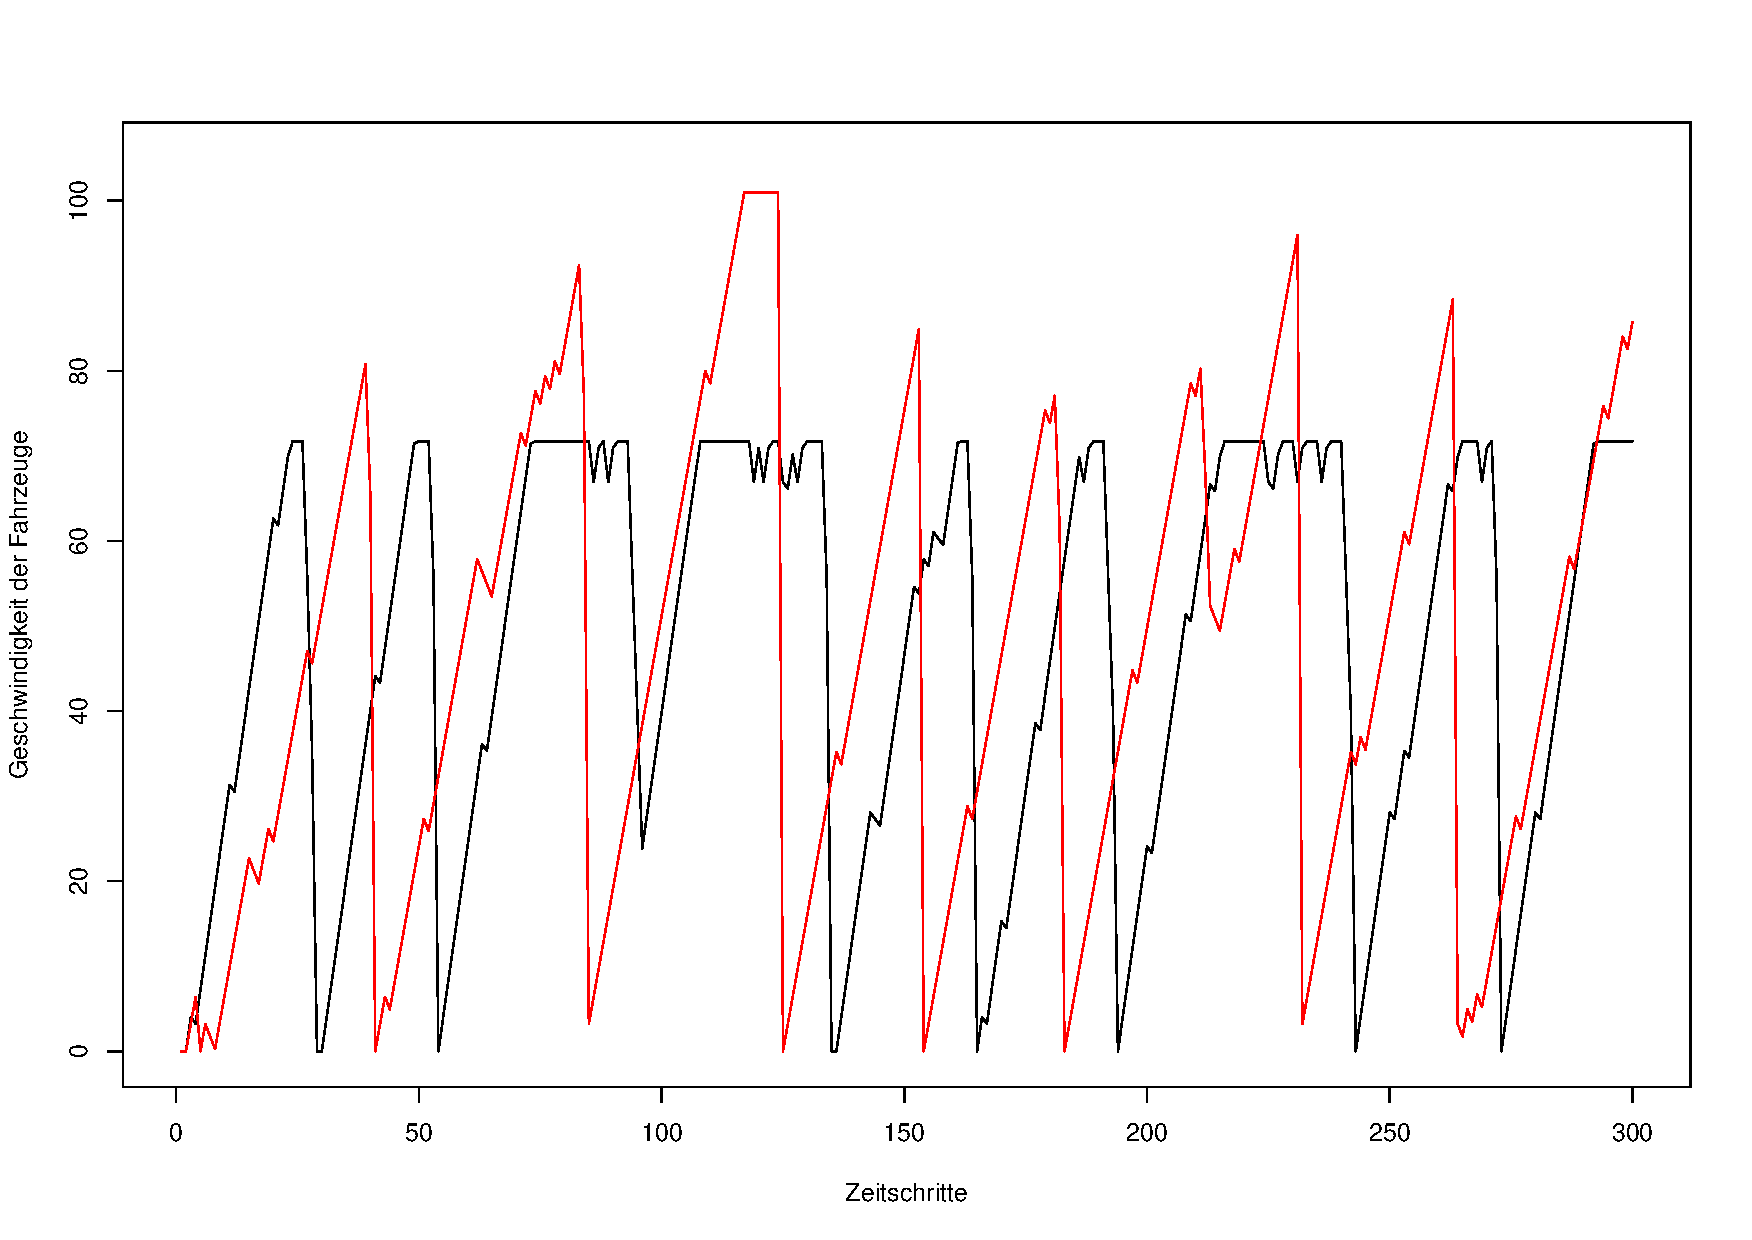
\includegraphics[width=0.3\textwidth]{speed_run1}}\qquad 
   \subfigure[2. Durchgang]{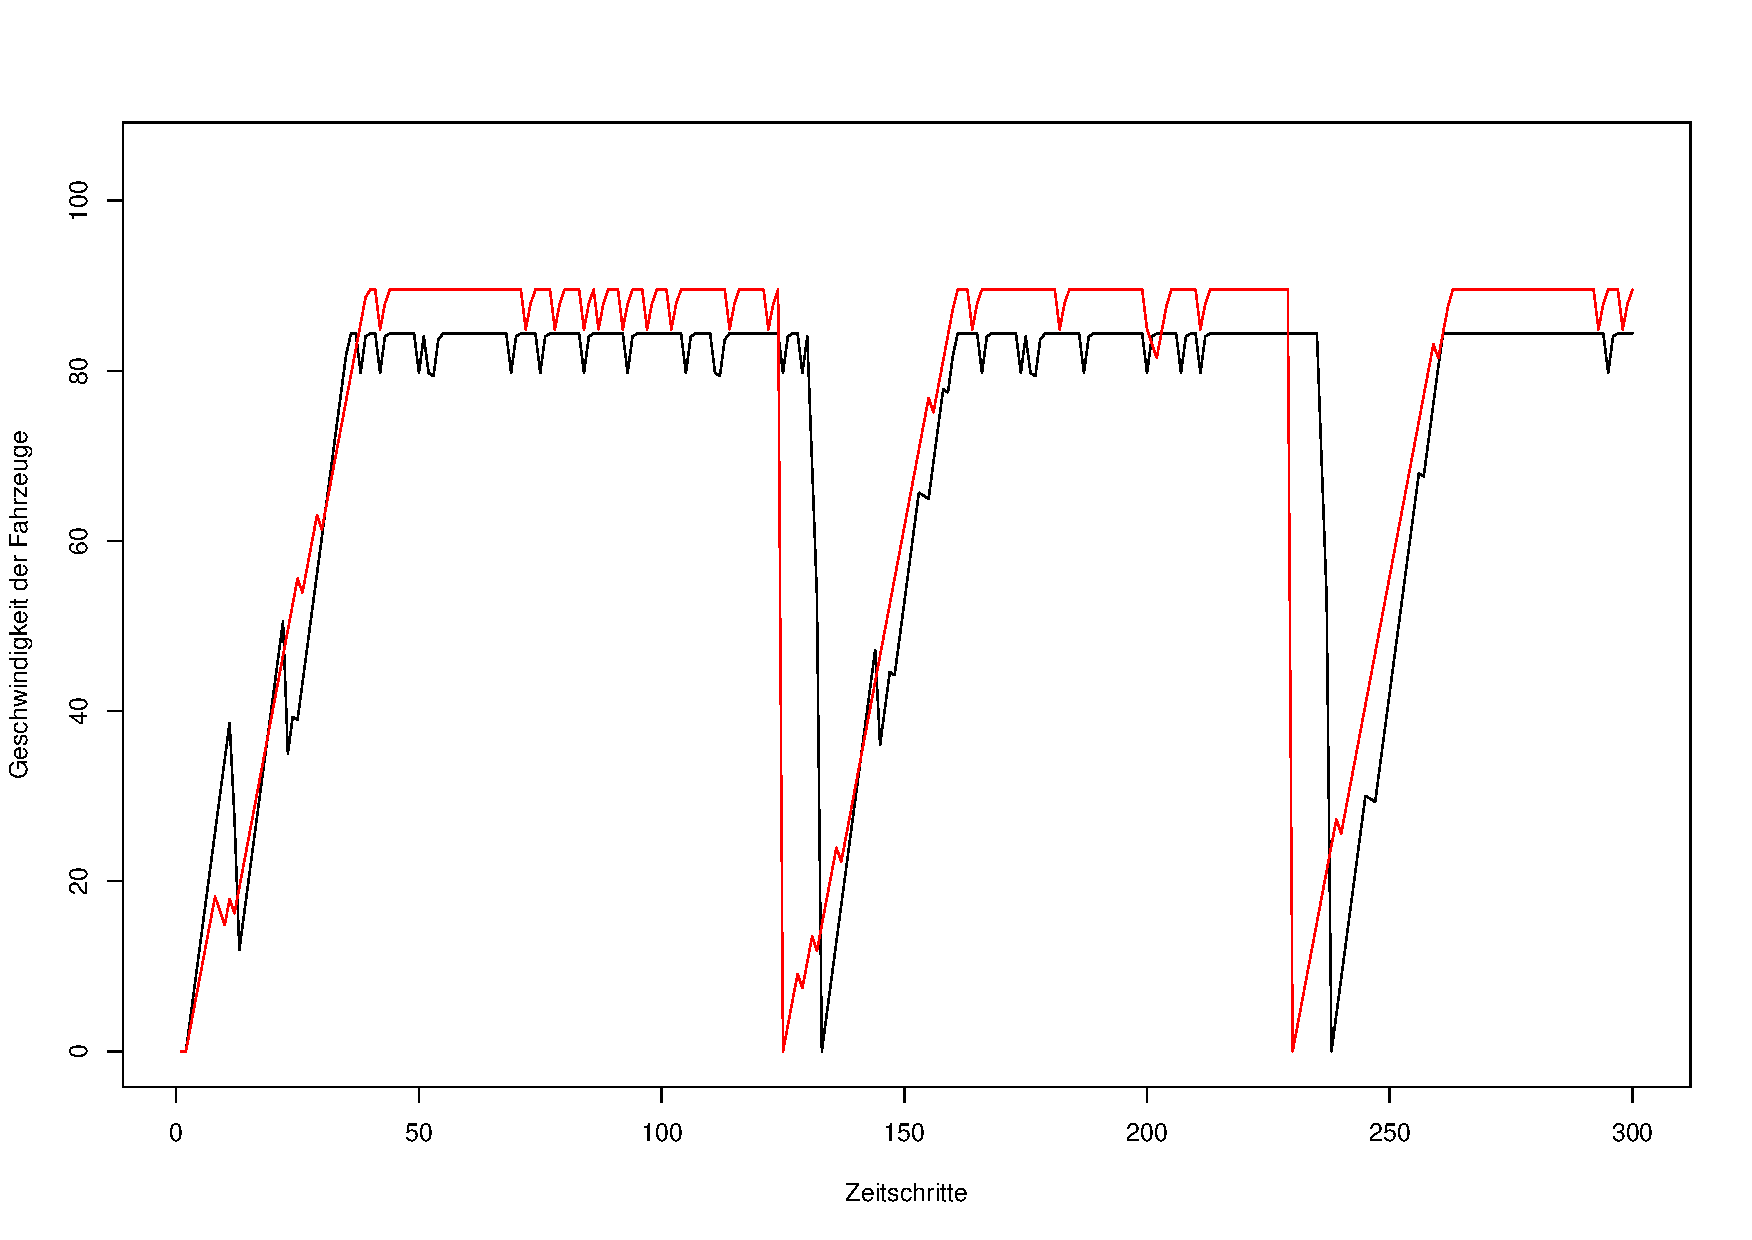
\includegraphics[width=0.3\textwidth]{speed_run2}}\qquad 
   \subfigure[3. Durchgang]{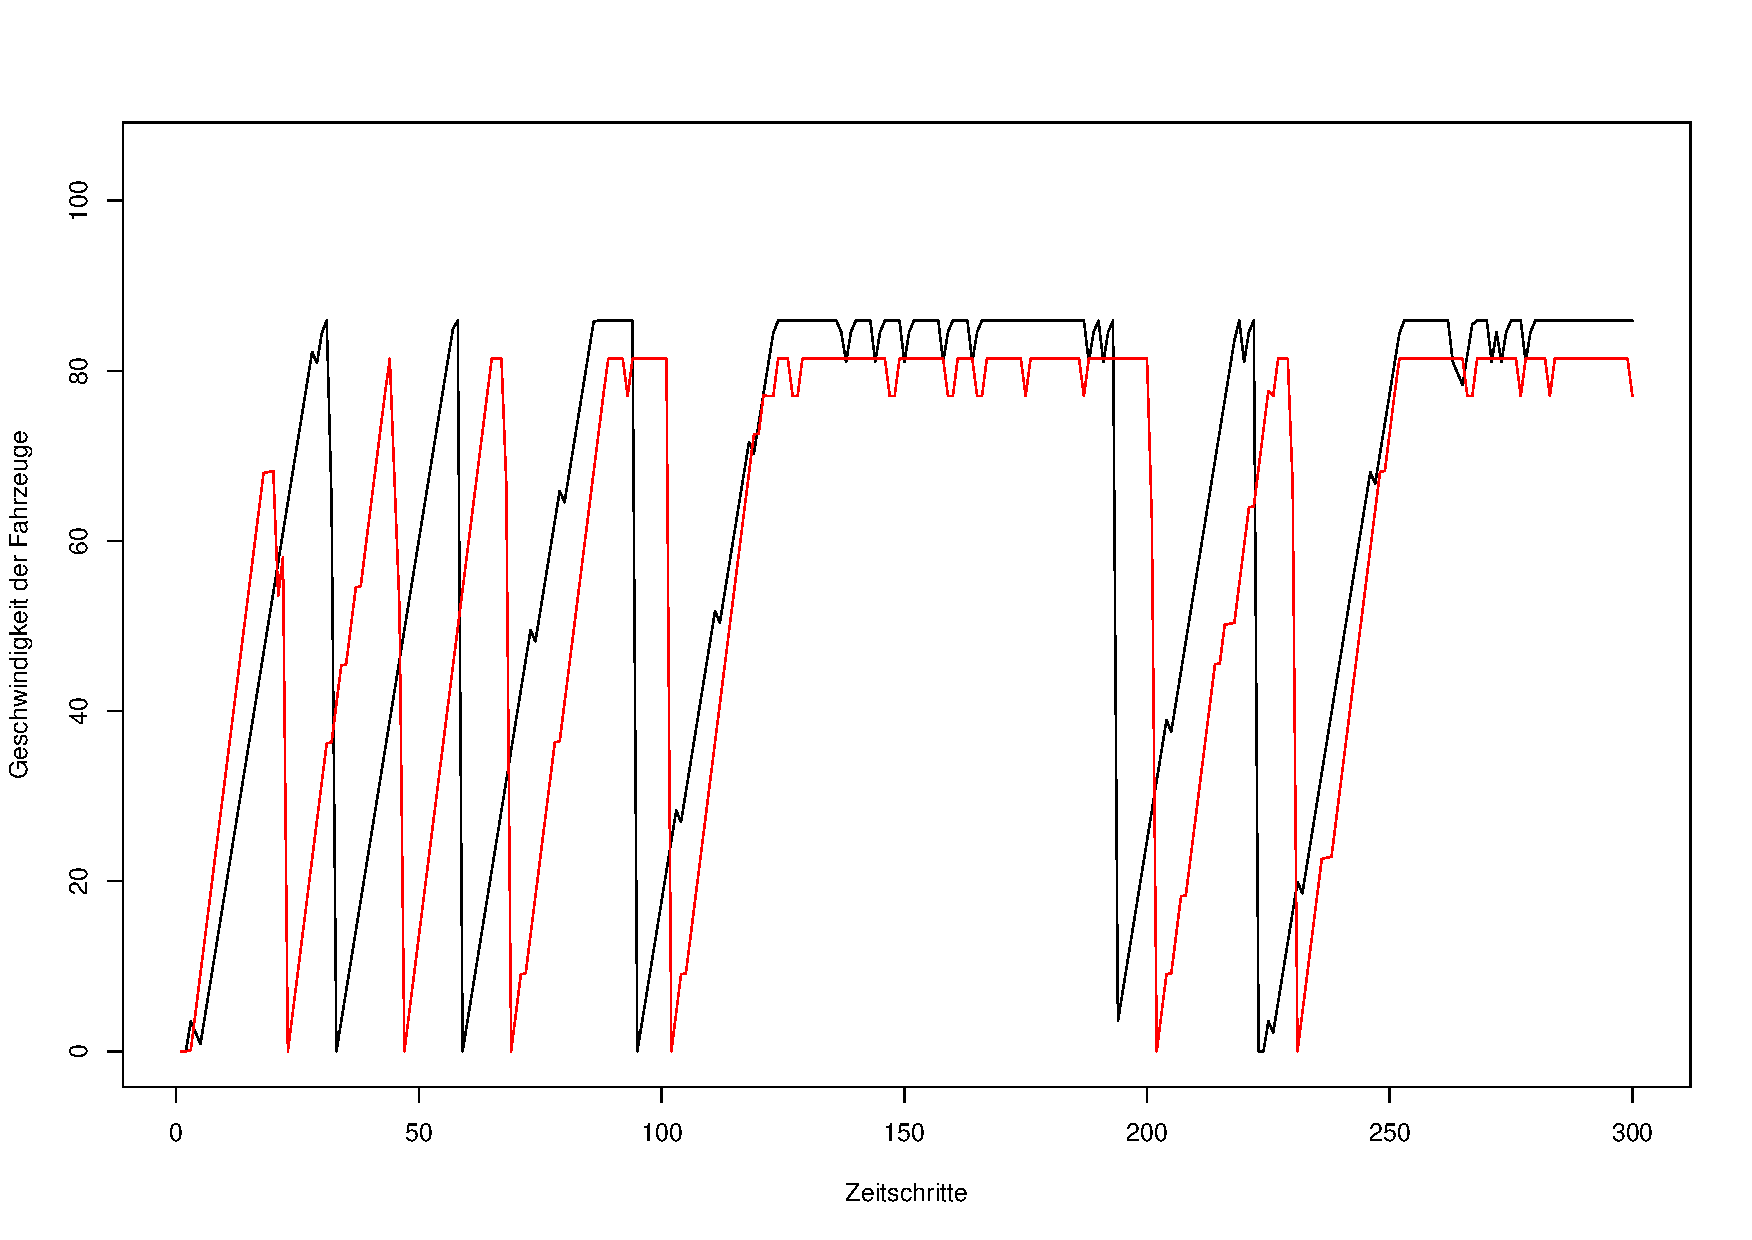
\includegraphics[width=0.3\textwidth]{speed_run3}}
  \caption{Simulationen mit Zellgröße 7,5 m und Zeitschrittlänge 0,1 min} 
  \label{figure:run1-3}
\end{figure}

In allen drei Kurvenverläufen in \cref{figure:run1-3} sind mehrfach Reduktionen der Geschwindigkeit auf Null zu sehen. 
Dies zeigt, dass an diesen Stellen eine Kollision stattgefunden hat. Das Kollisionsereignis wird vom Simulationstool ausgelöst, wenn ein Fahrzeug nicht in der Lage wäre, im nächsten Zeitschritt die für seine Geschwindigkeit entsprechende Streckenlänge zurückzulegen.

Die Zeitschrittlänge von 0,1 Minuten, was sechs Sekunden entspricht, ist nicht ausreichend, um Geschwindigkeit in ausreichendem Maße abzubauen, um genug Abstand vom Vordermann einzuhalten.

Auf die Ausführung von Durchgängen mit dieser Zeitschrittgröße und kleinerer Zellgröße wurde verzichtet.

\begin{figure}[hptb]
  \centering 
   \subfigure[1. Durchgang]{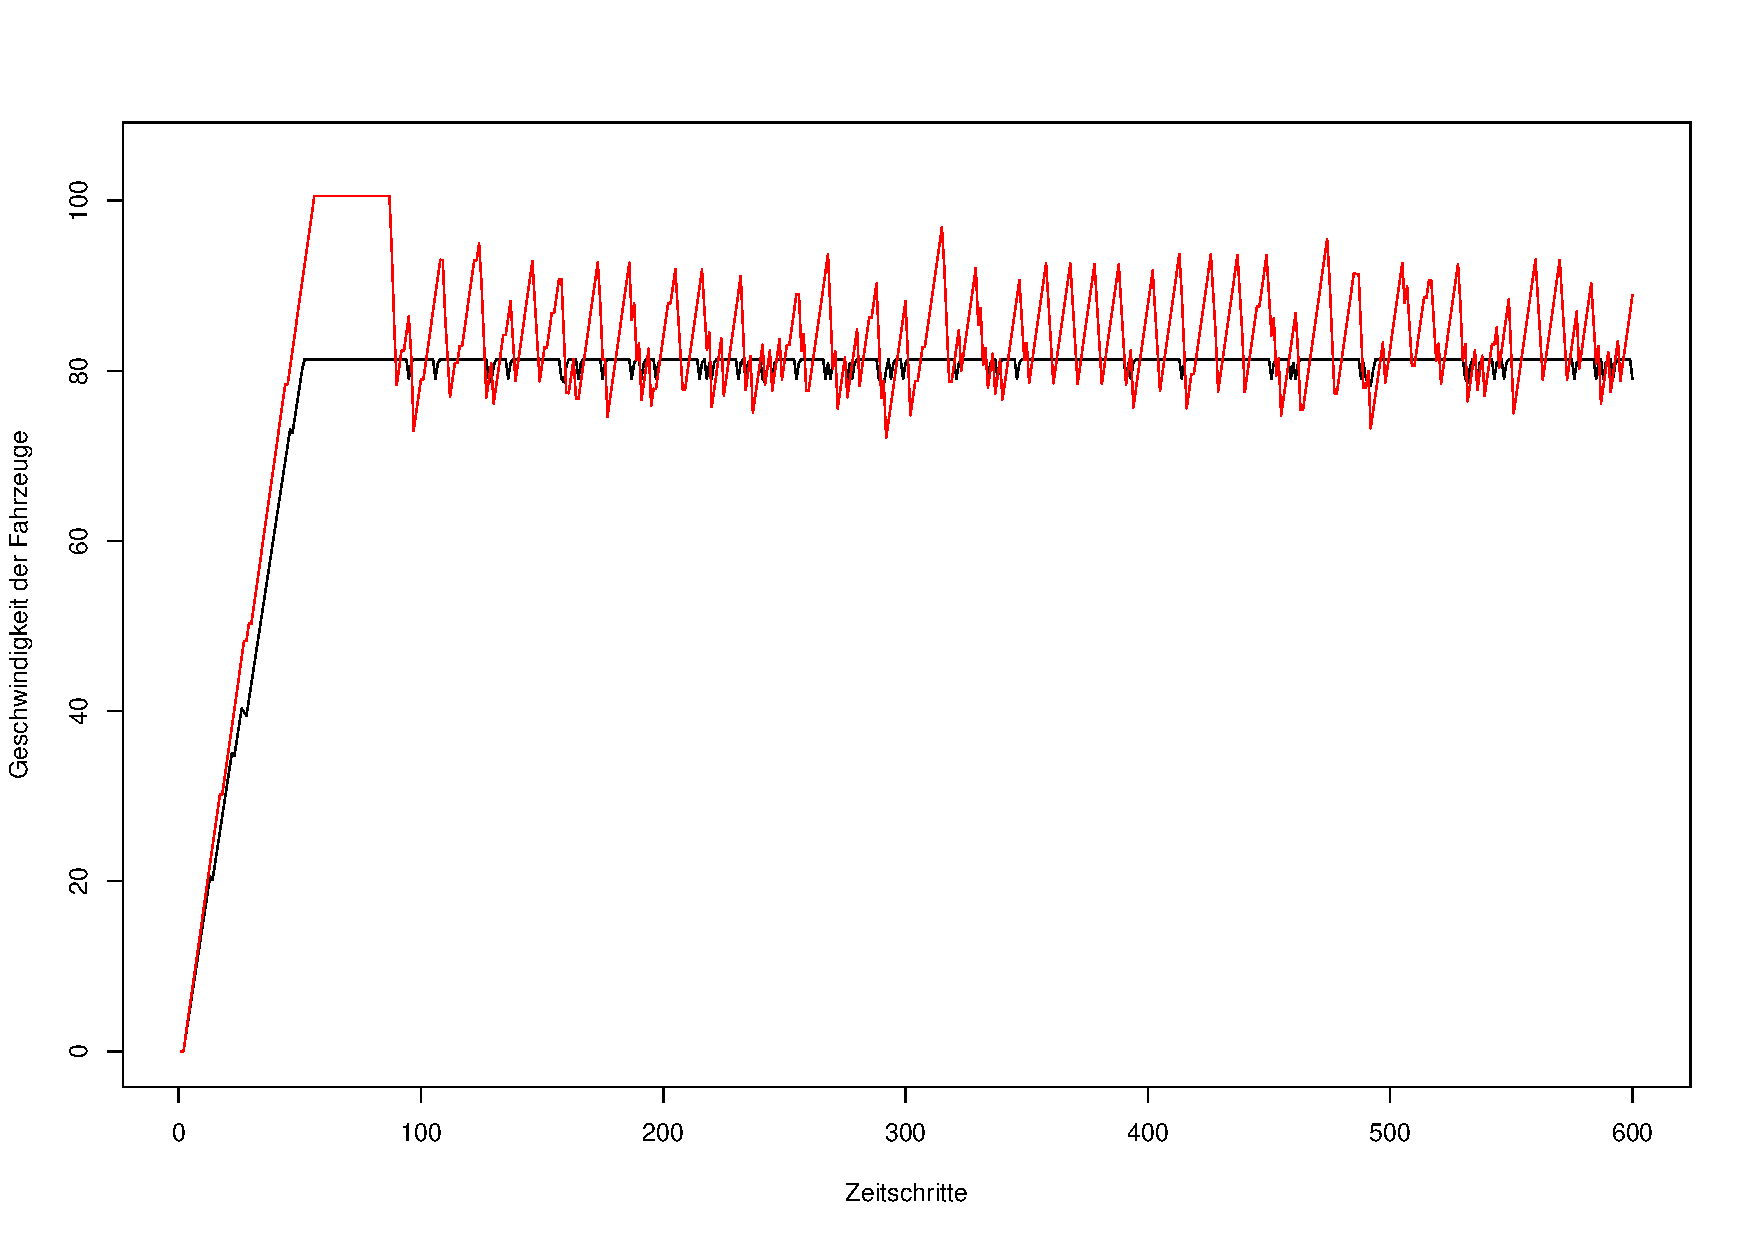
\includegraphics[width=0.3\textwidth]{speed_run4}}\qquad 
   \subfigure[2. Durchgang]{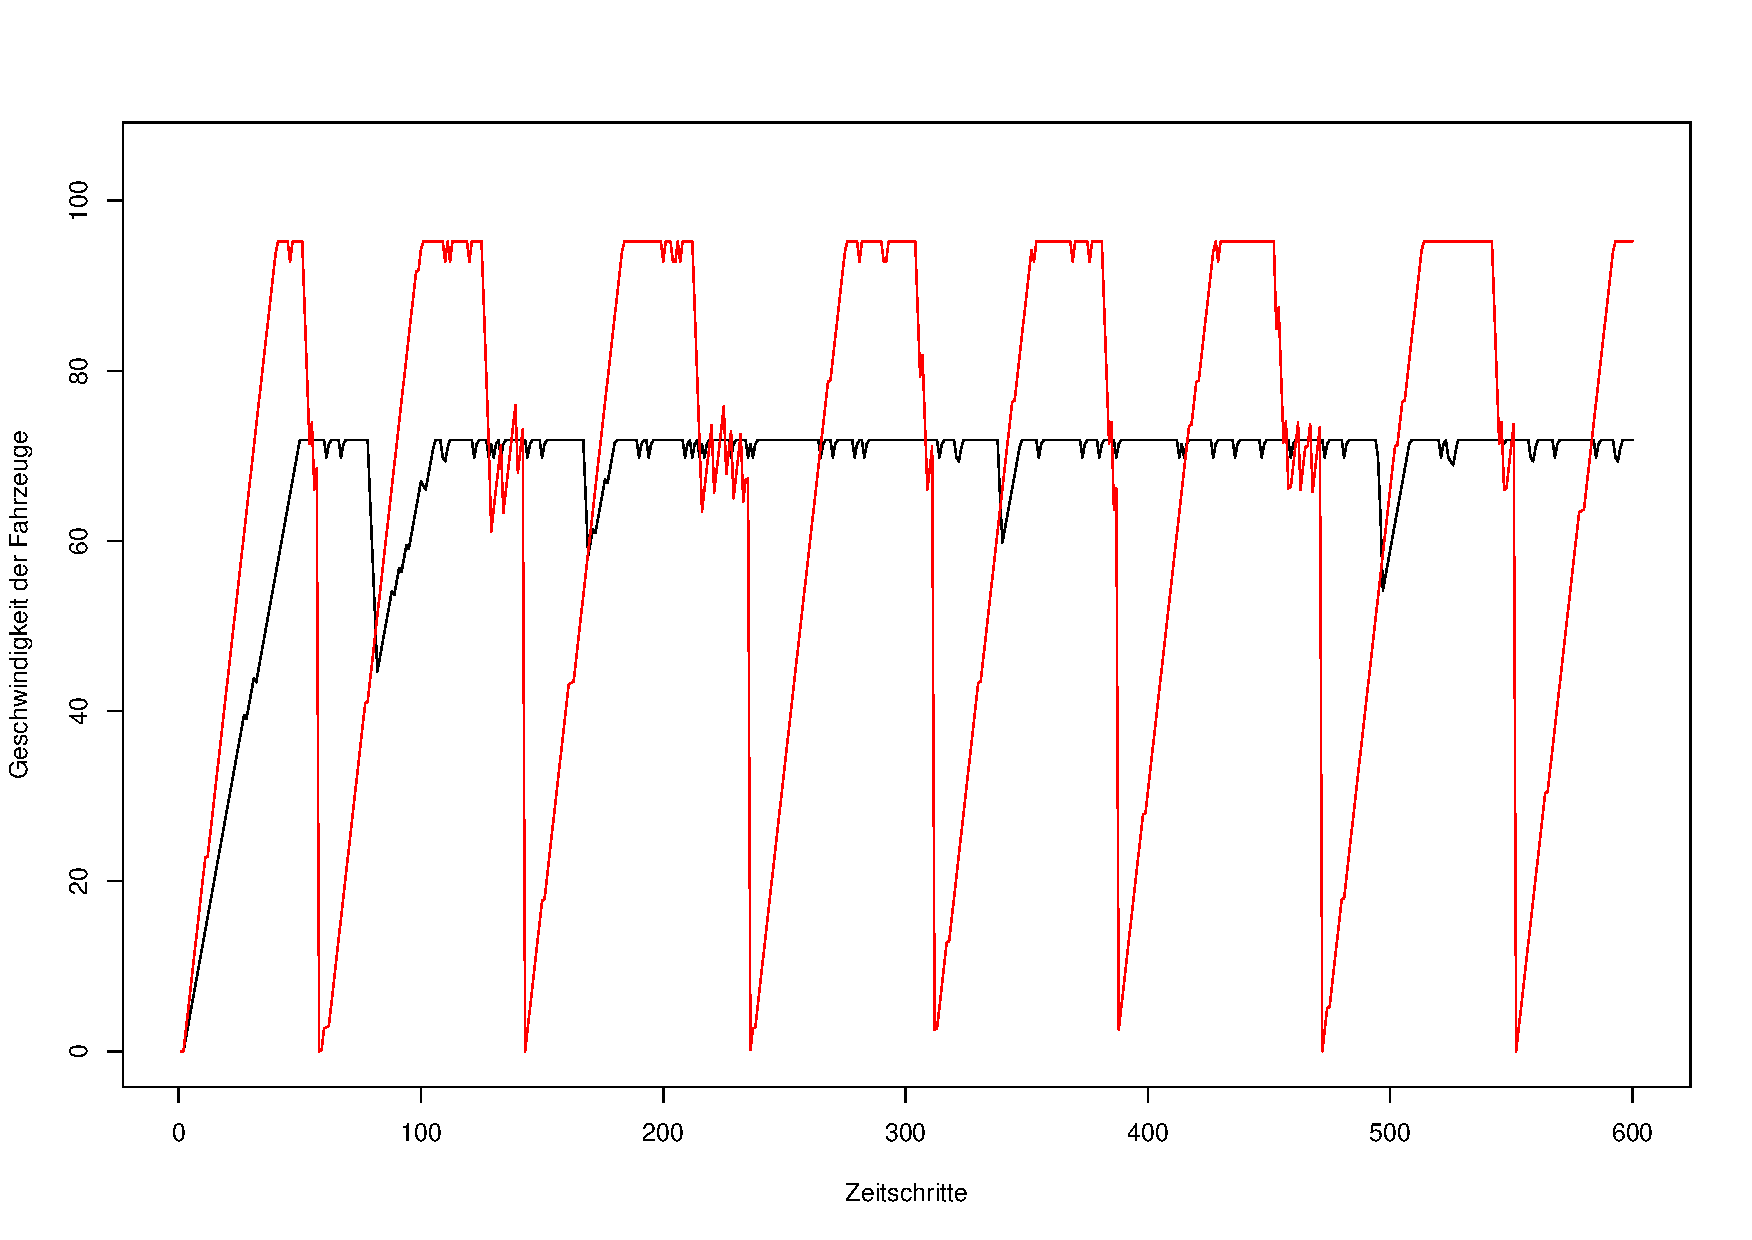
\includegraphics[width=0.3\textwidth]{speed_run5}}\qquad 
   \subfigure[3. Durchgang]{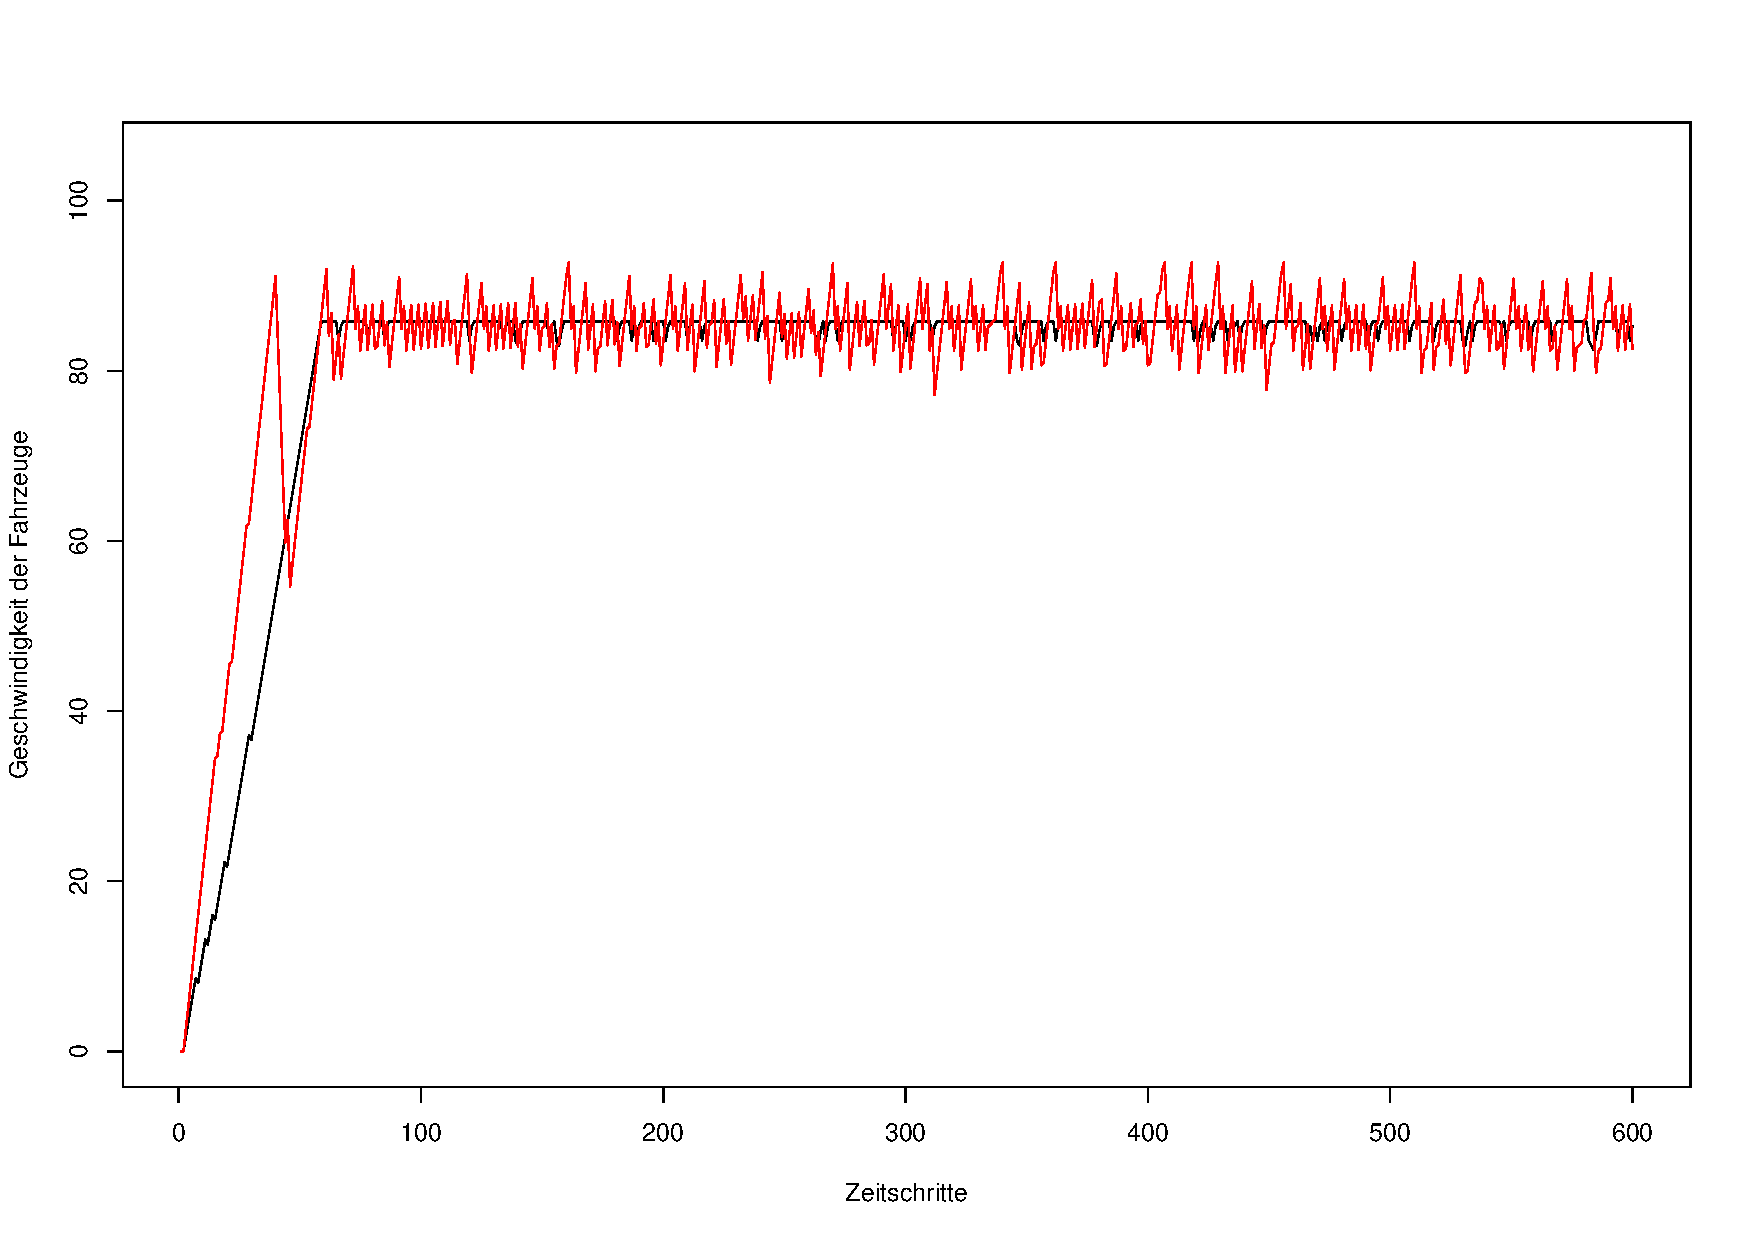
\includegraphics[width=0.3\textwidth]{speed_run6}}
  \caption{Simulationen mit Zellgröße 7,5 m und Zeitschrittlänge 0,05 min} 
  \label{figure:run4-6}
\end{figure}

Die Verläufe der Kurven in \cref{figure:run4-6} zeigen in zwei von drei Fällen, dass sich die Geschwindigkeit des auffahrenden Fahrzeuges um die des langsameren Fahrzeuges einpendelt.

Das Plot des zweiten Durchganges zeigt, dass auch in dieser Konstellation eine Kollision stattgefunden hat.
Die Geschwindigkeit des langsameren Fahrzeuges lag in diesem Durchgang in Vergleich zu den anderen beiden um einiges niedriger, sodass die Zeiträume zwischen den Eingriffsmöglichkeiten zu hoch waren.

\begin{figure}[hptb]
  \centering 
   \subfigure[1. Durchgang]{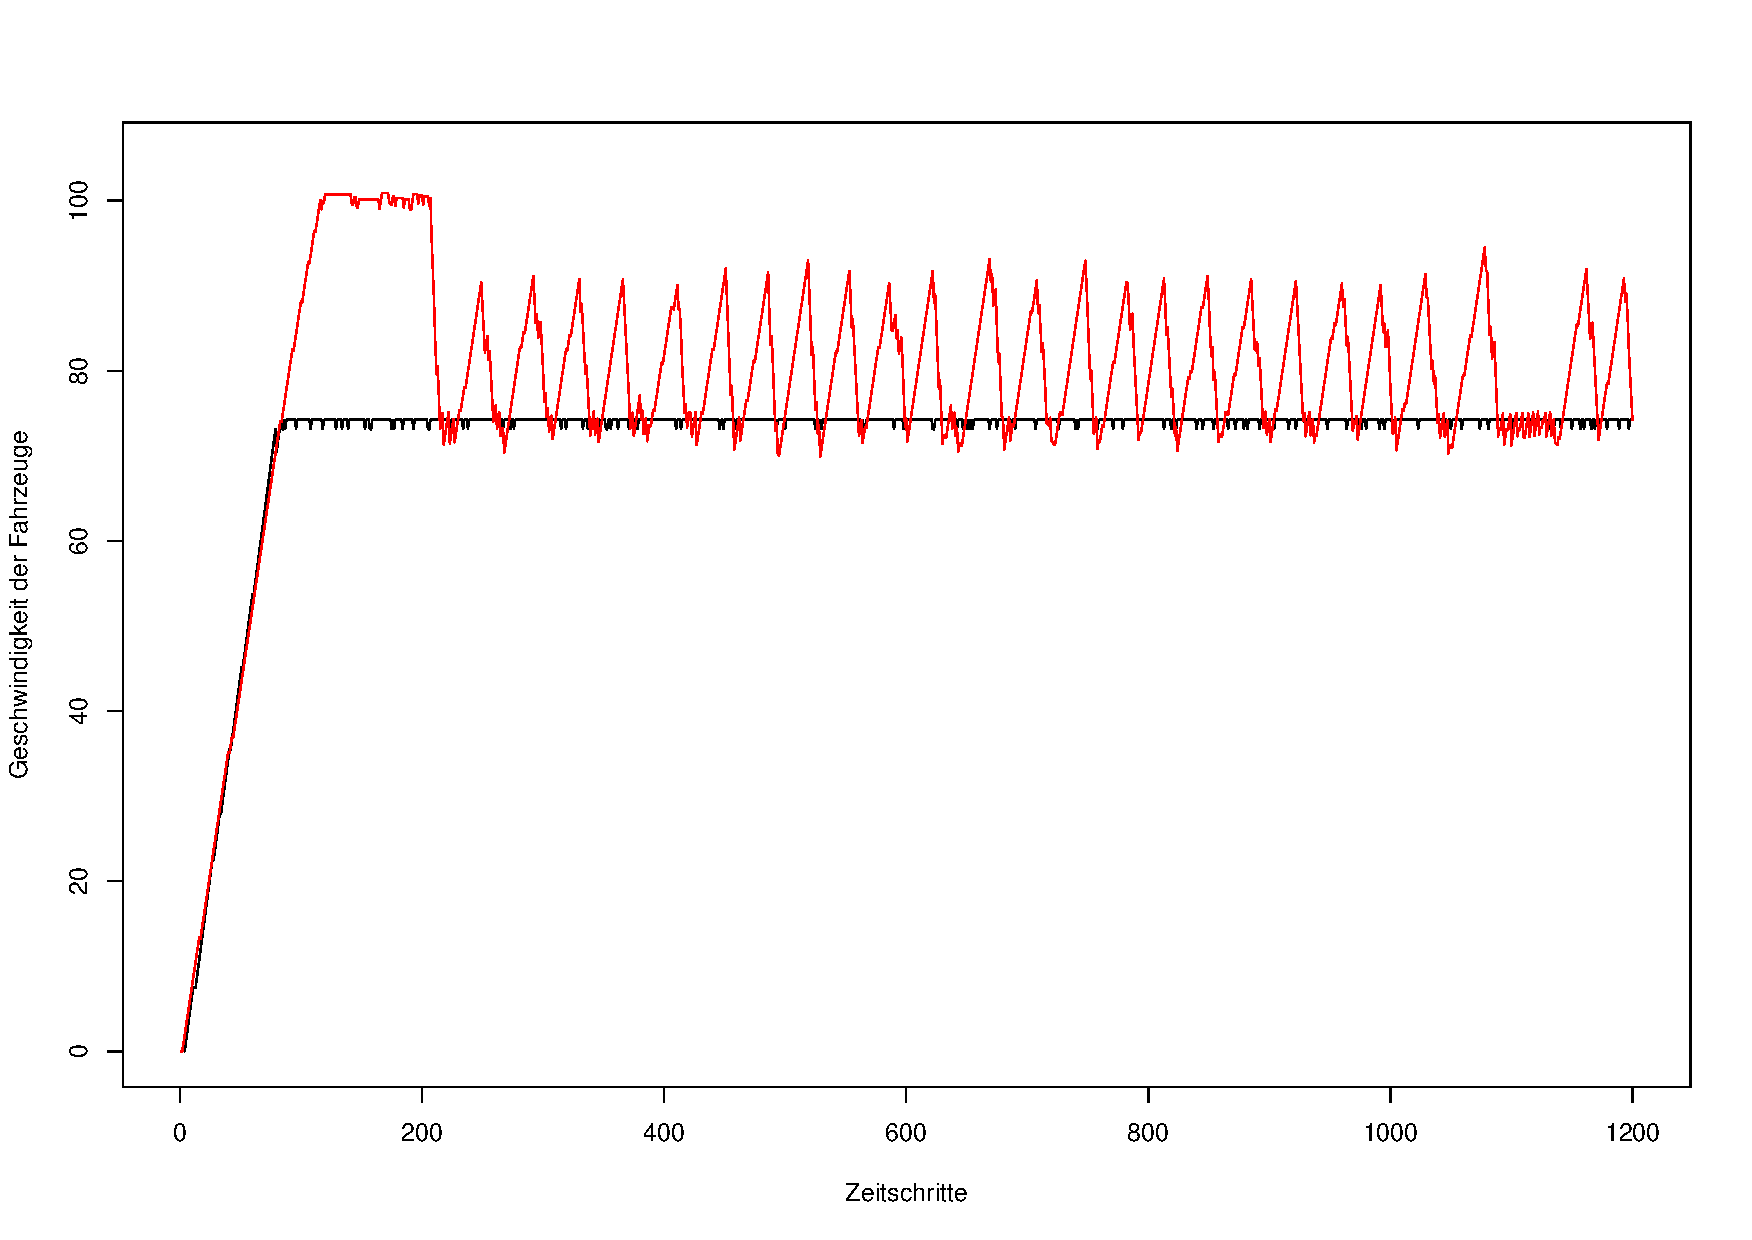
\includegraphics[width=0.3\textwidth]{speed_run7}}\qquad 
   \subfigure[2. Durchgang]{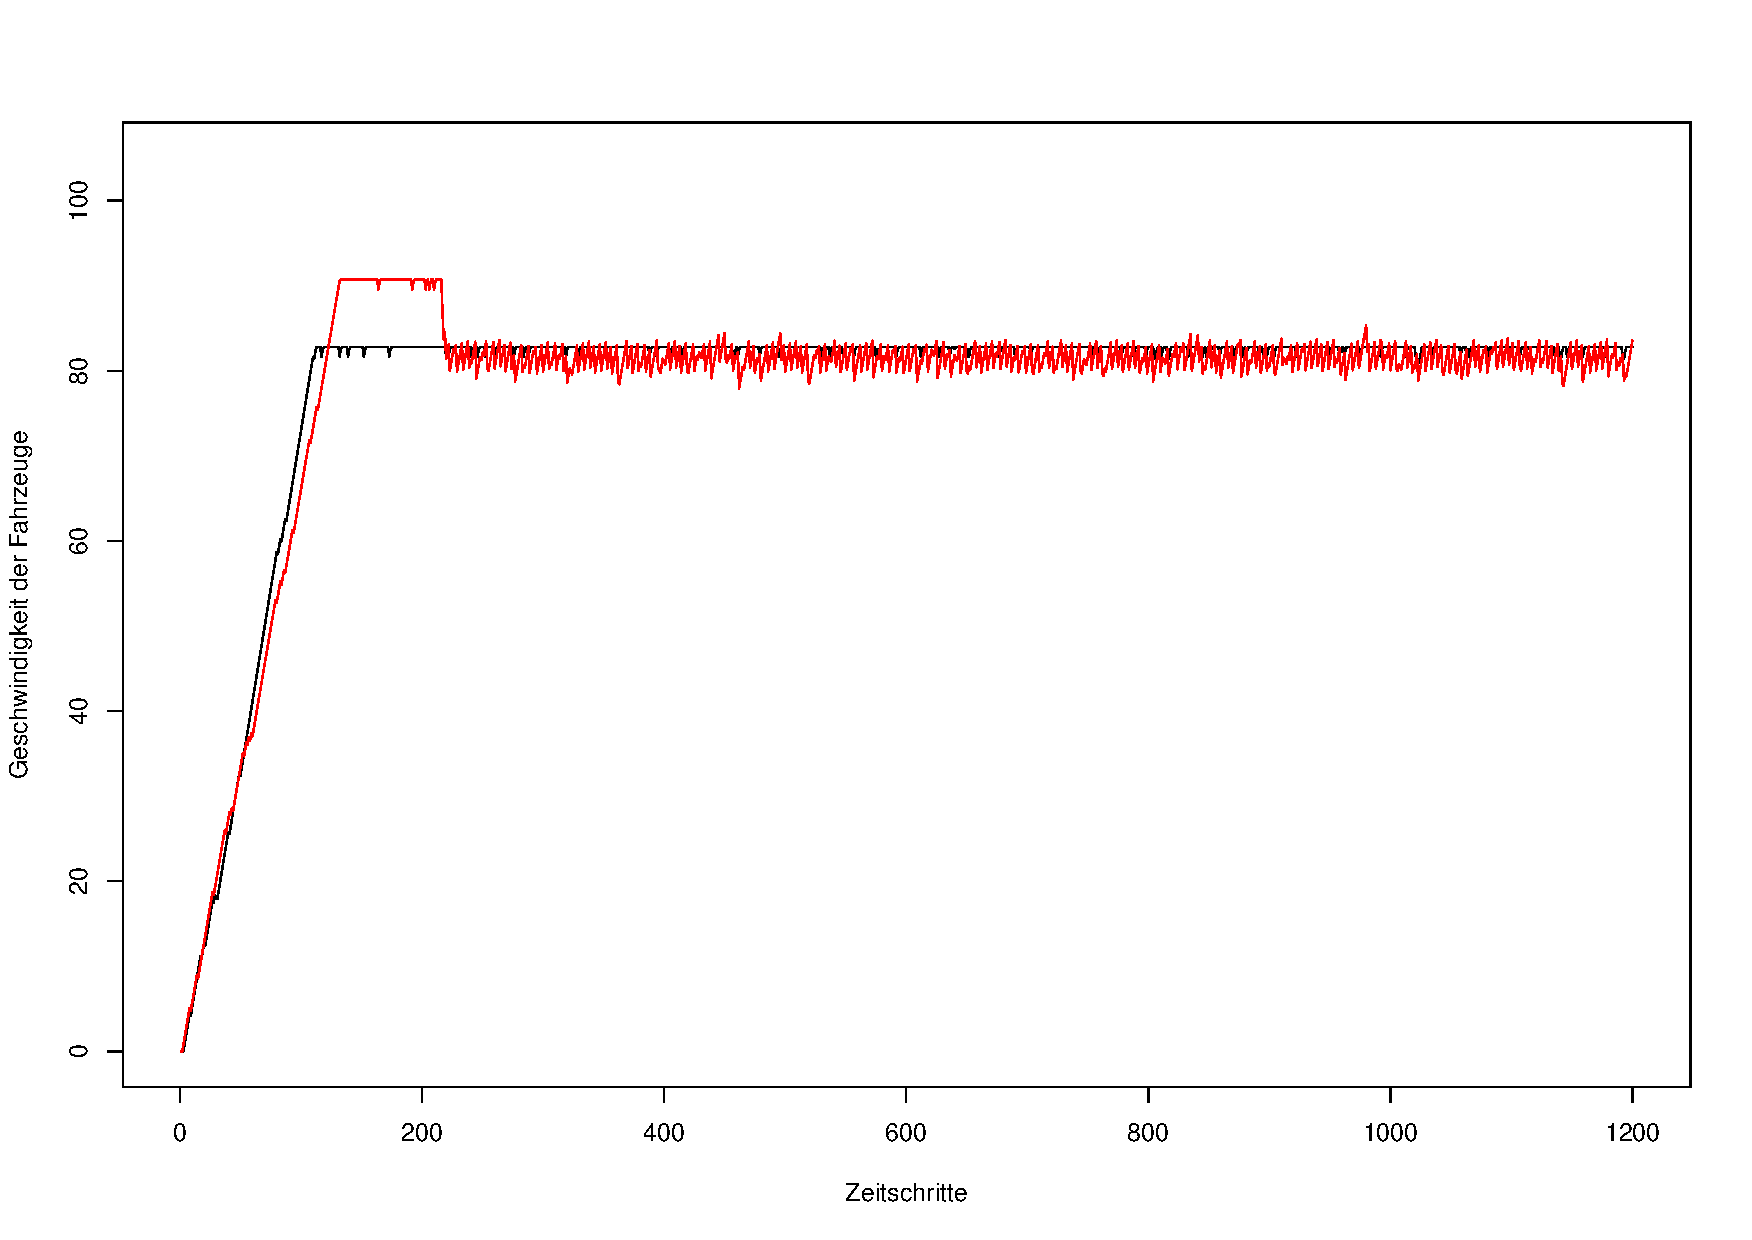
\includegraphics[width=0.3\textwidth]{speed_run8}}\qquad 
   \subfigure[3. Durchgang]{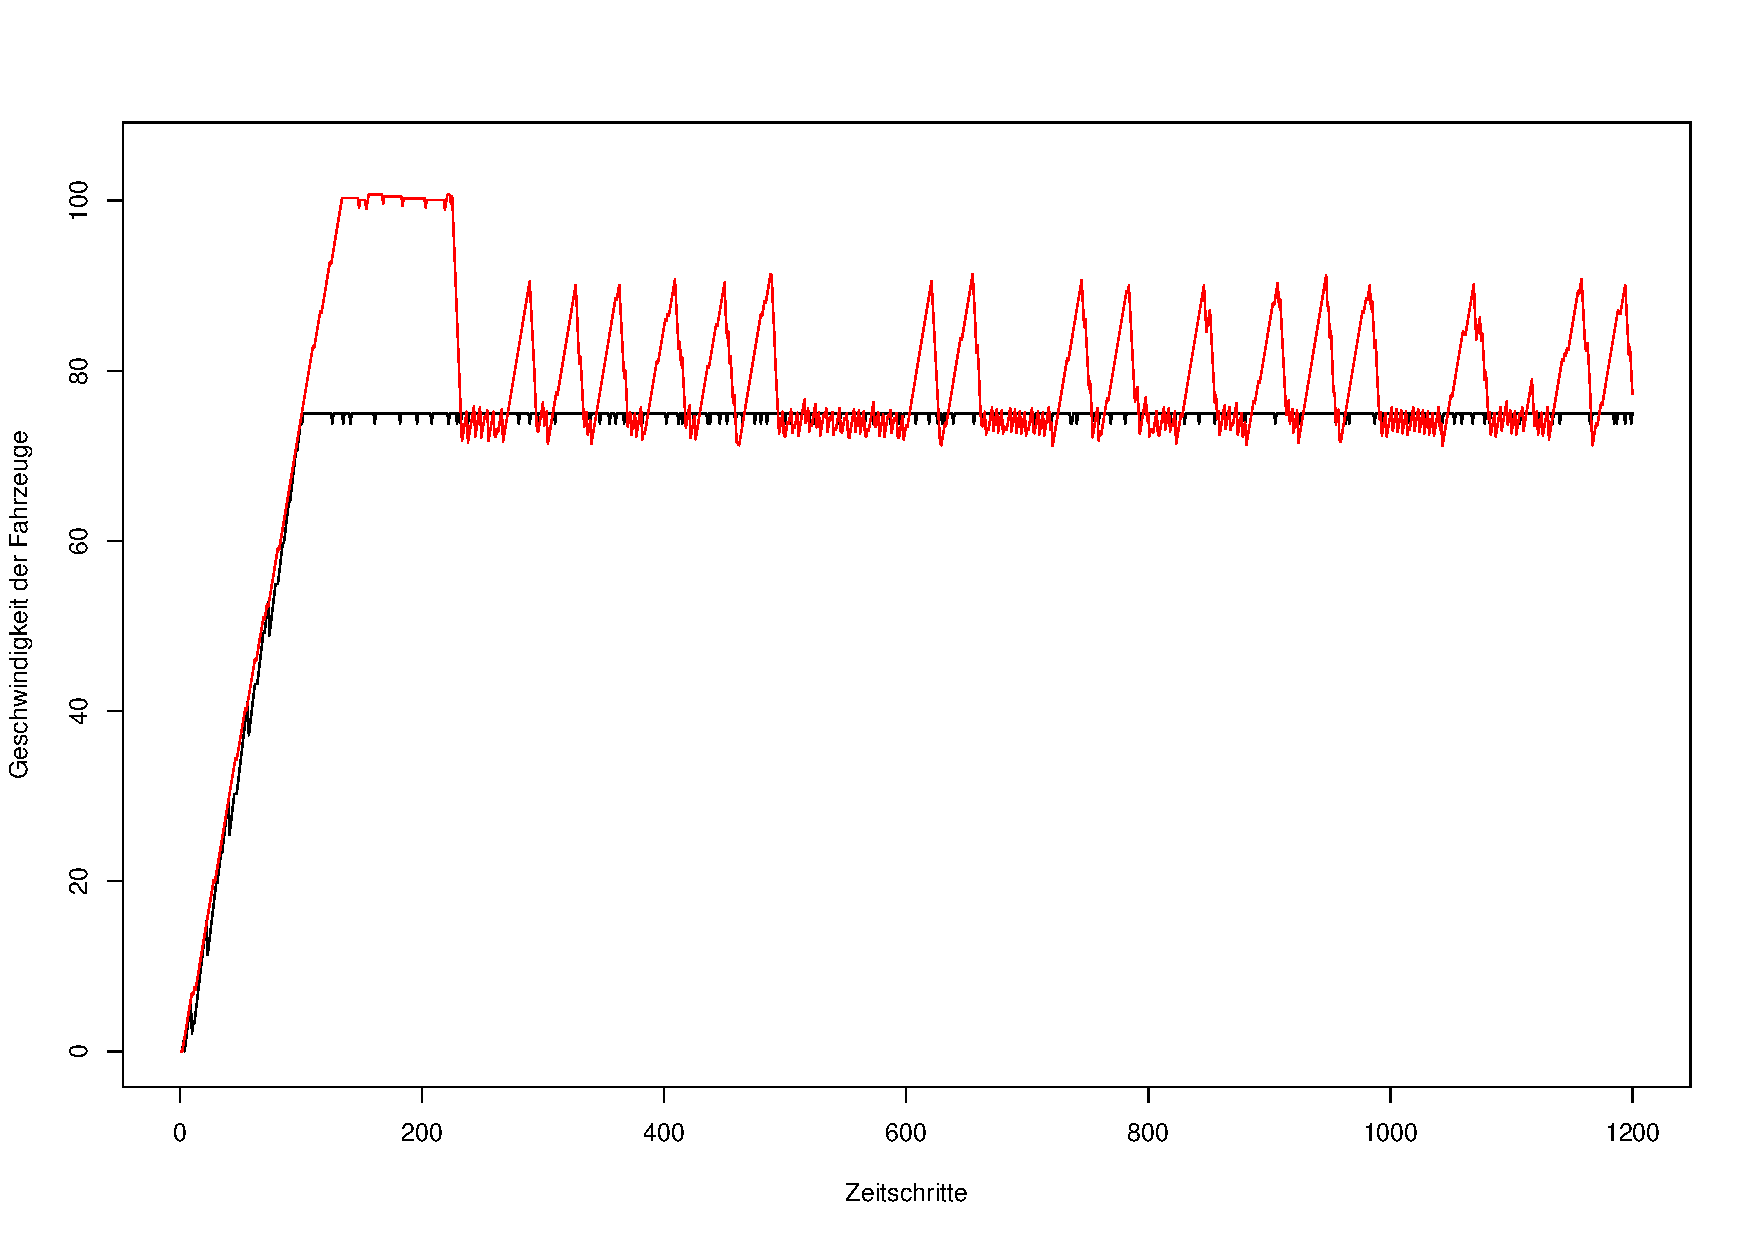
\includegraphics[width=0.3\textwidth]{speed_run9}}
  \caption{Simulationen mit Zellgröße 7,5 m und Zeitschrittlänge 0,025 min} 
  \label{figure:run7-8}
\end{figure}

Die Geschwindigkeitskurve des schnelleren Fahrzeugs weist in \cref{figure:run7-9}(a) ein sägezahnähnliches Muster auf.
Dies resultiert aus den, im Vergleich zu den herbeigeführten Geschwindigkeitszuwächsen, großen Zellen.
Ein Geschwindigkeitsunterschied von zehn bis 15 km/h reicht bei entsprechend zugrunde liegender Ausgangsgeschwindigkeit nicht aus, eine Verkürzung des Abstands herbeizuführen.
Da sich die Abbrems- und Beschleunigungsmanöver identisch wiederholen, kommt es zu dieser Musterbildung.

Plot (b) zeigt ein Einordnen hinter dem langsameren Fahrzeug und die Beibehaltung dessen Geschwindigkeit.
Plot (c) ist nahezu eine Mischform aus den ersten beiden Kurven.

\subsubsection{Zellgröße 5,0 m}

\begin{figure}[hptb]
  \centering 
   \subfigure[1. Durchgang]{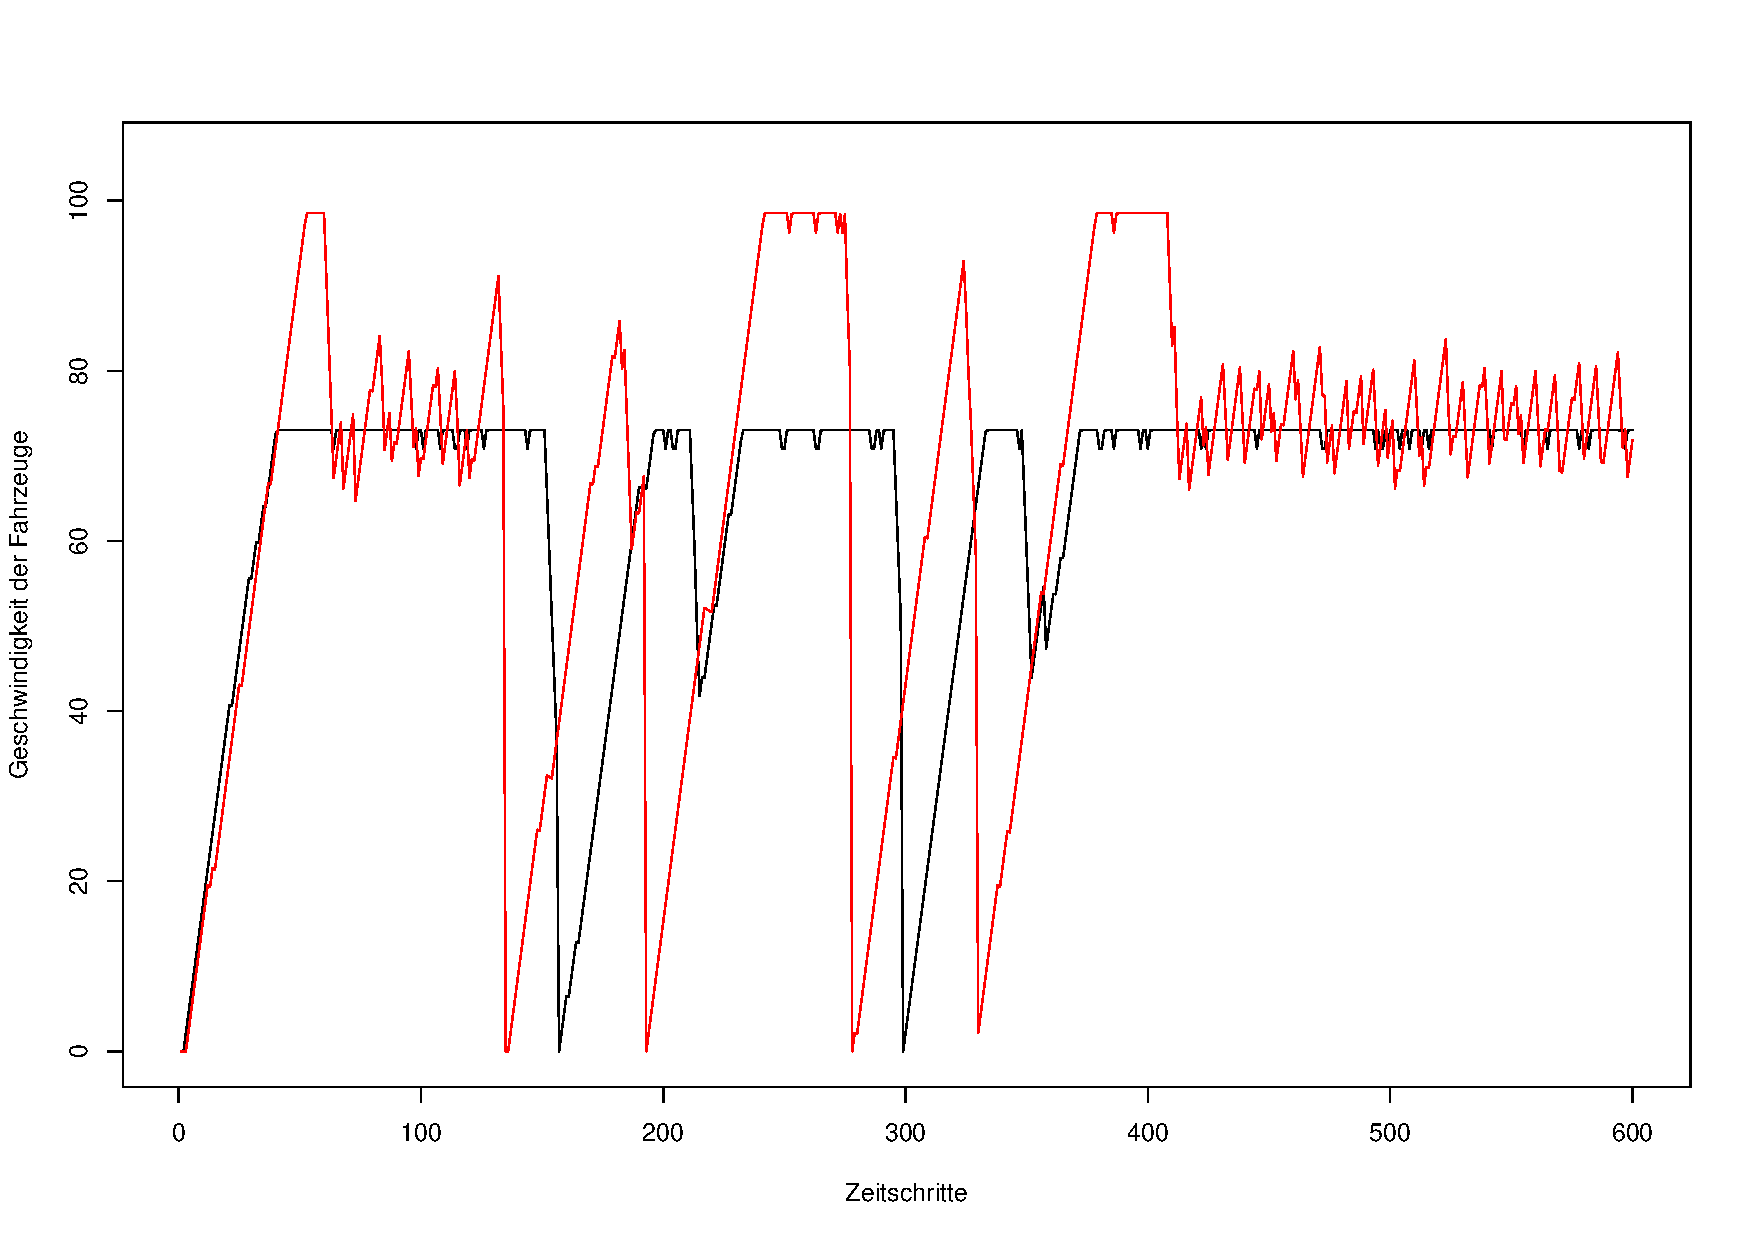
\includegraphics[width=0.3\textwidth]{speed_run14}}\qquad 
   \subfigure[2. Durchgang]{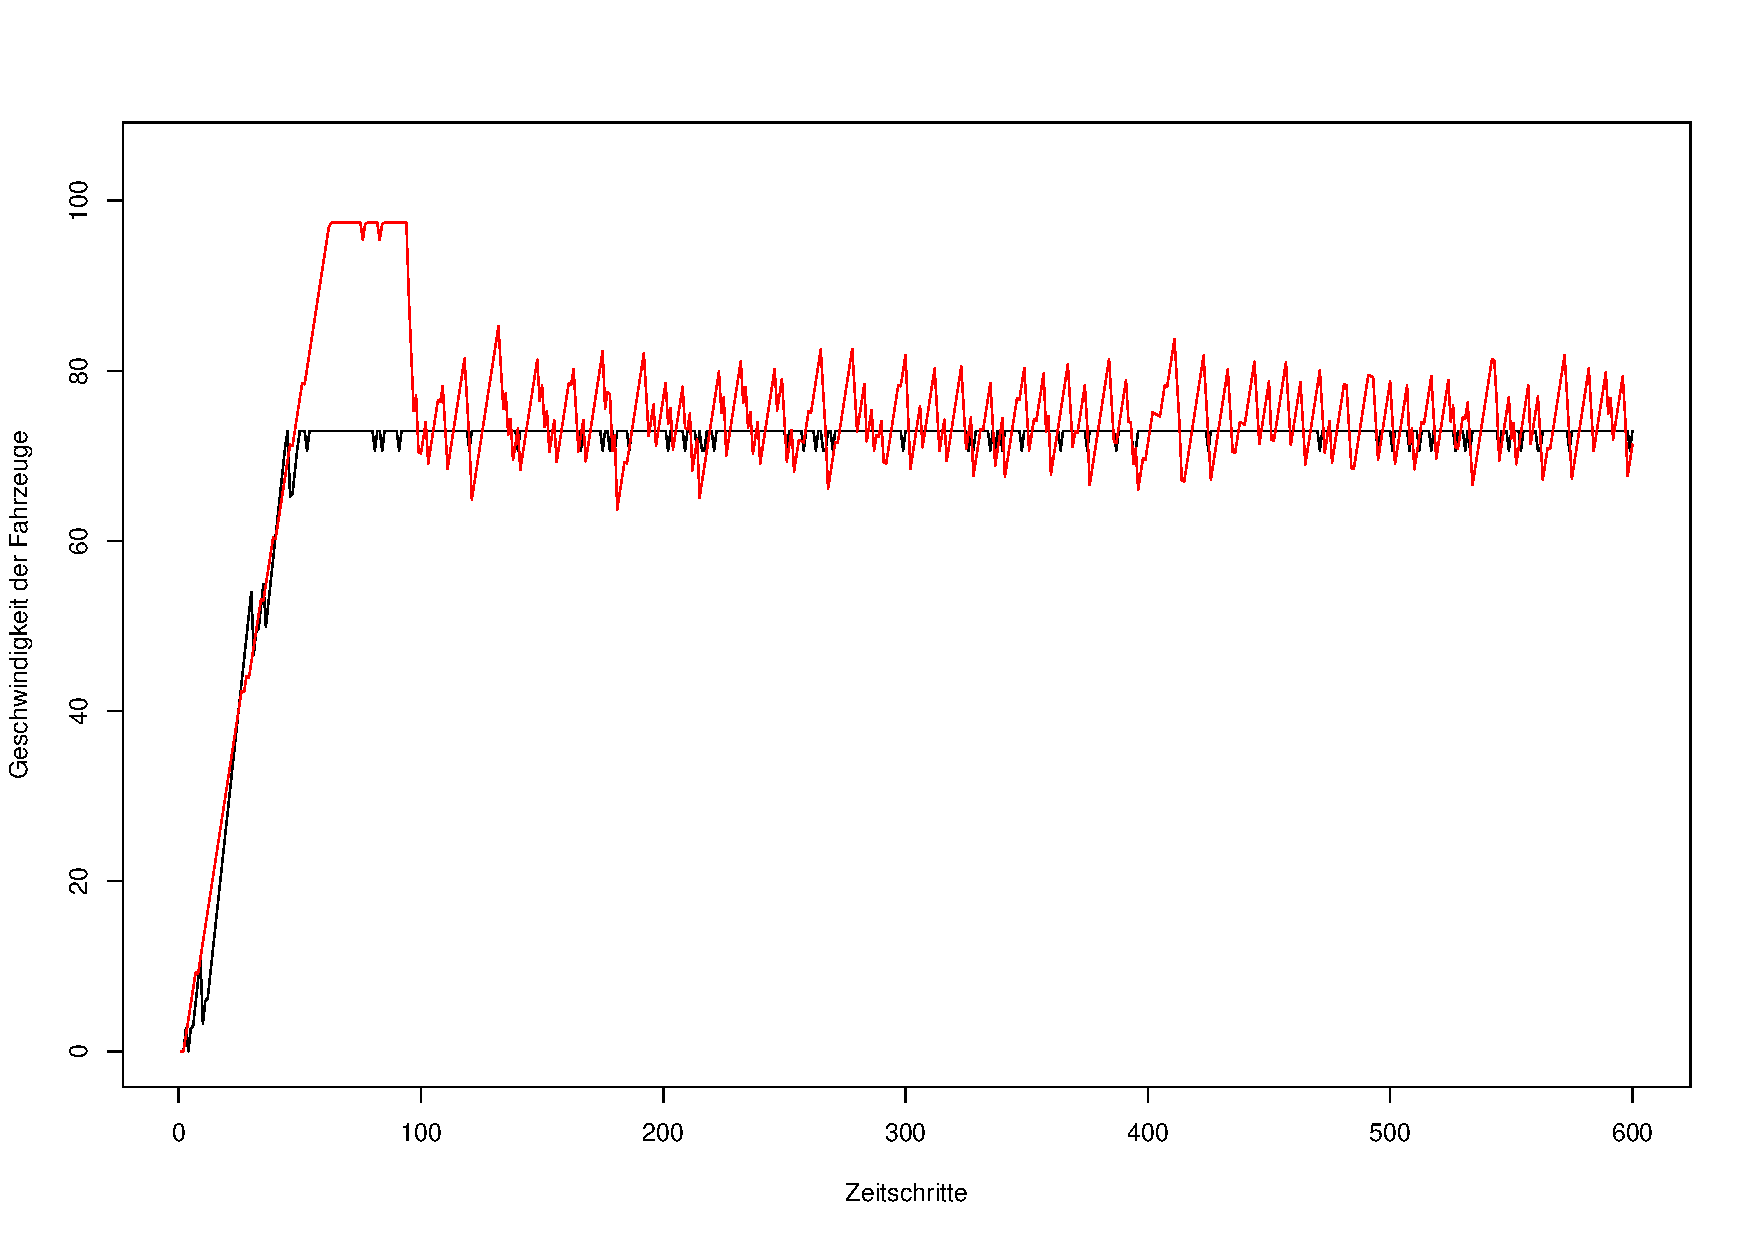
\includegraphics[width=0.3\textwidth]{speed_run15}}\qquad 
   \subfigure[3. Durchgang]{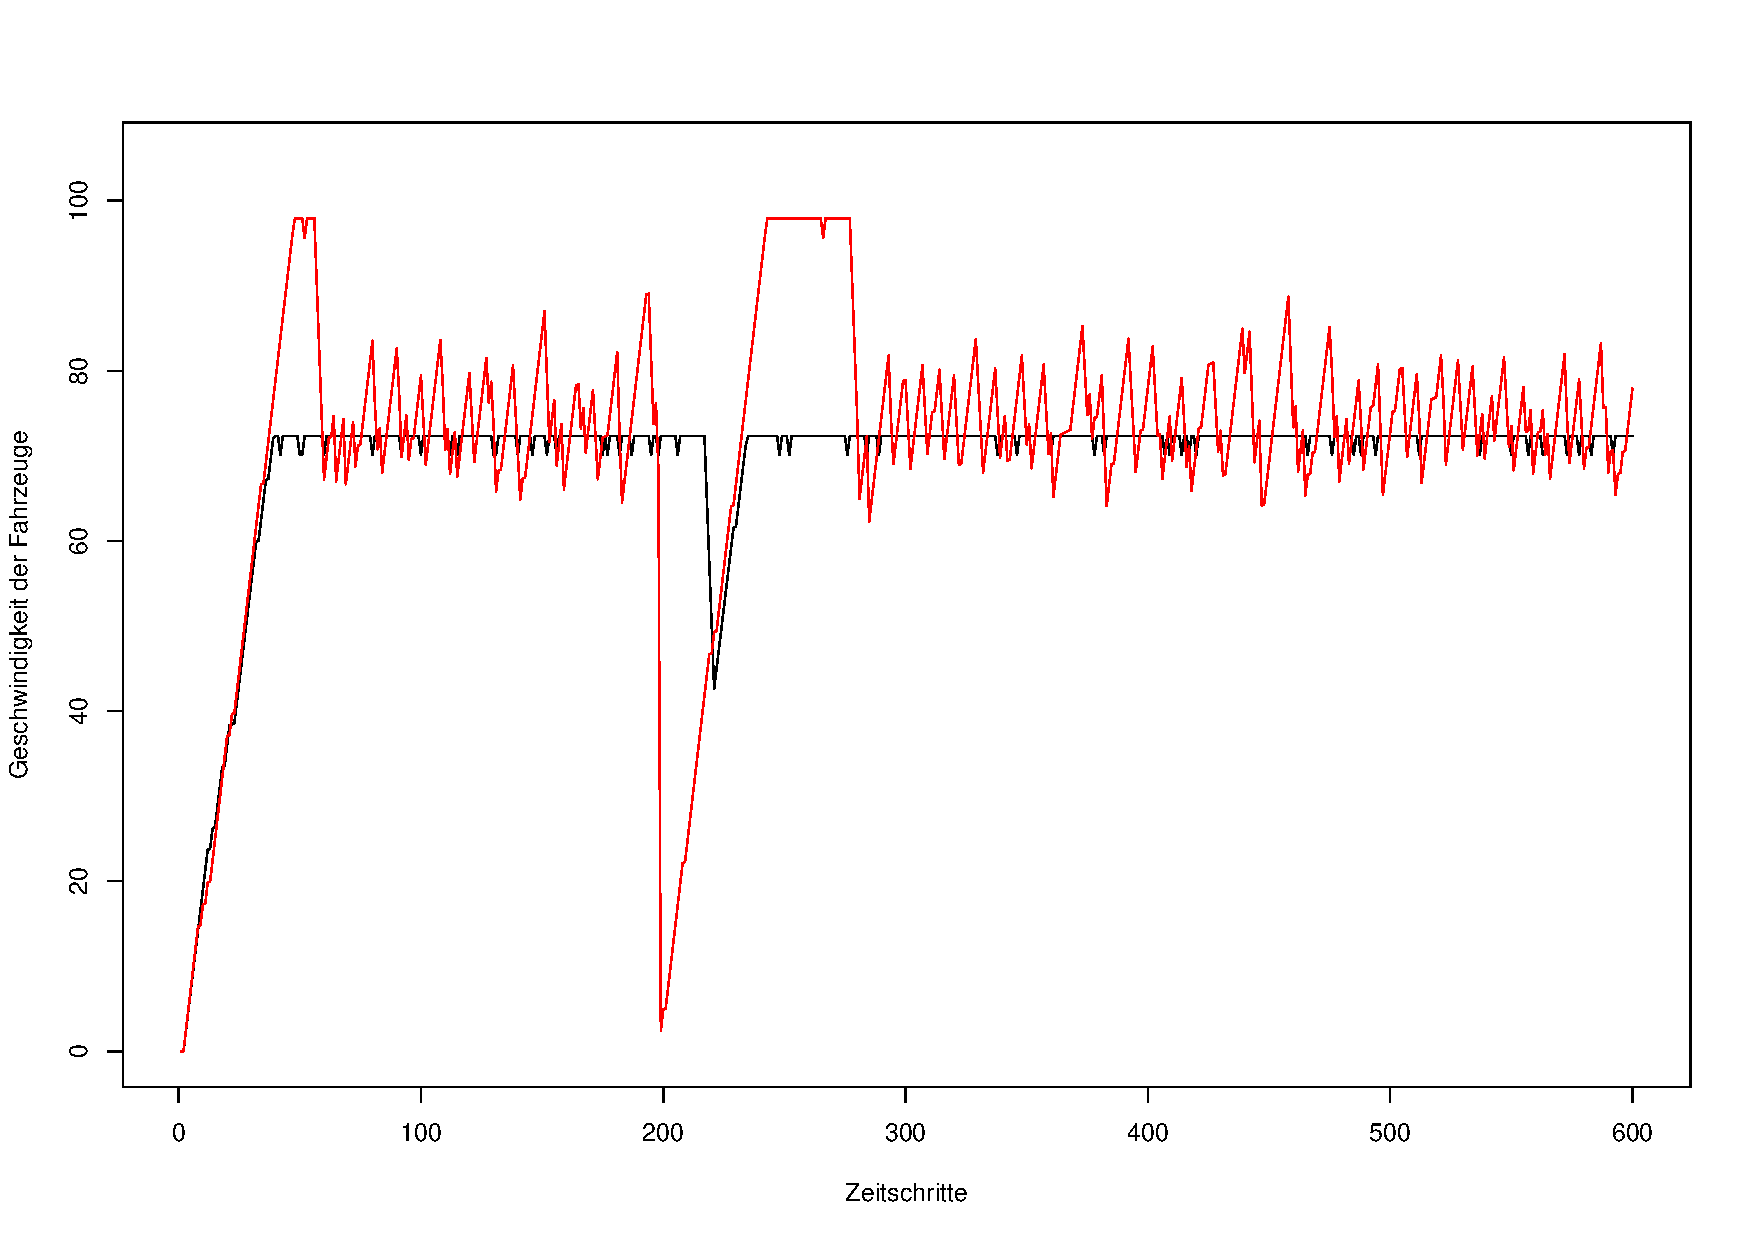
\includegraphics[width=0.3\textwidth]{speed_run16}}
  \caption{Simulationen mit Zellgröße 5,0 m und Zeitschrittlänge 0,05 min} 
  \label{figure:run14-16}
\end{figure}

Die Diagramme in \cref{figure:run14-16} zeigen wiederholt, dass der Abstand, der für den Bremsvorgang zur Verfügung steht, mit einem recht langen Zeitraum zwischen den Zeitschritten, nicht ausreicht.

\begin{figure}[hptb]
  \centering 
   \subfigure[1. Durchgang]{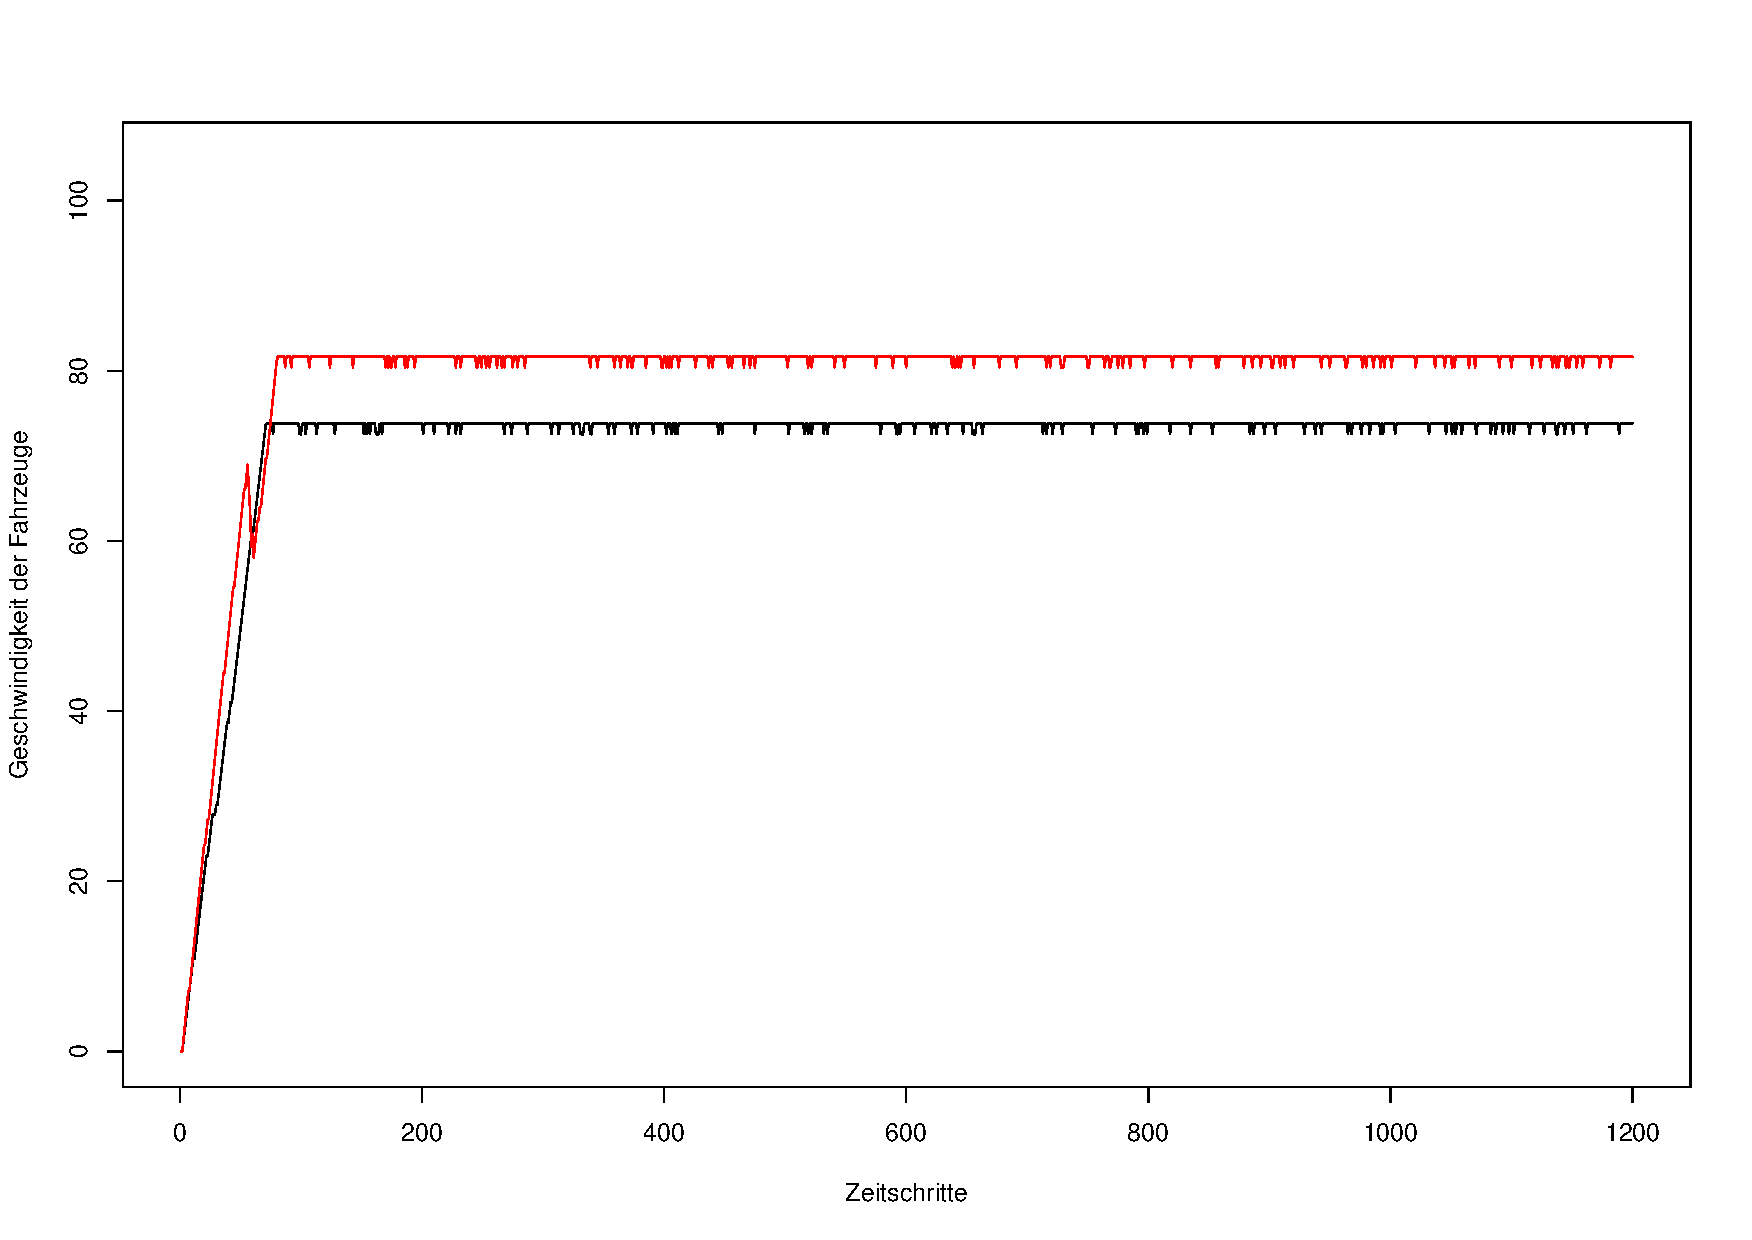
\includegraphics[width=0.3\textwidth]{speed_run17}}\qquad 
   \subfigure[2. Durchgang]{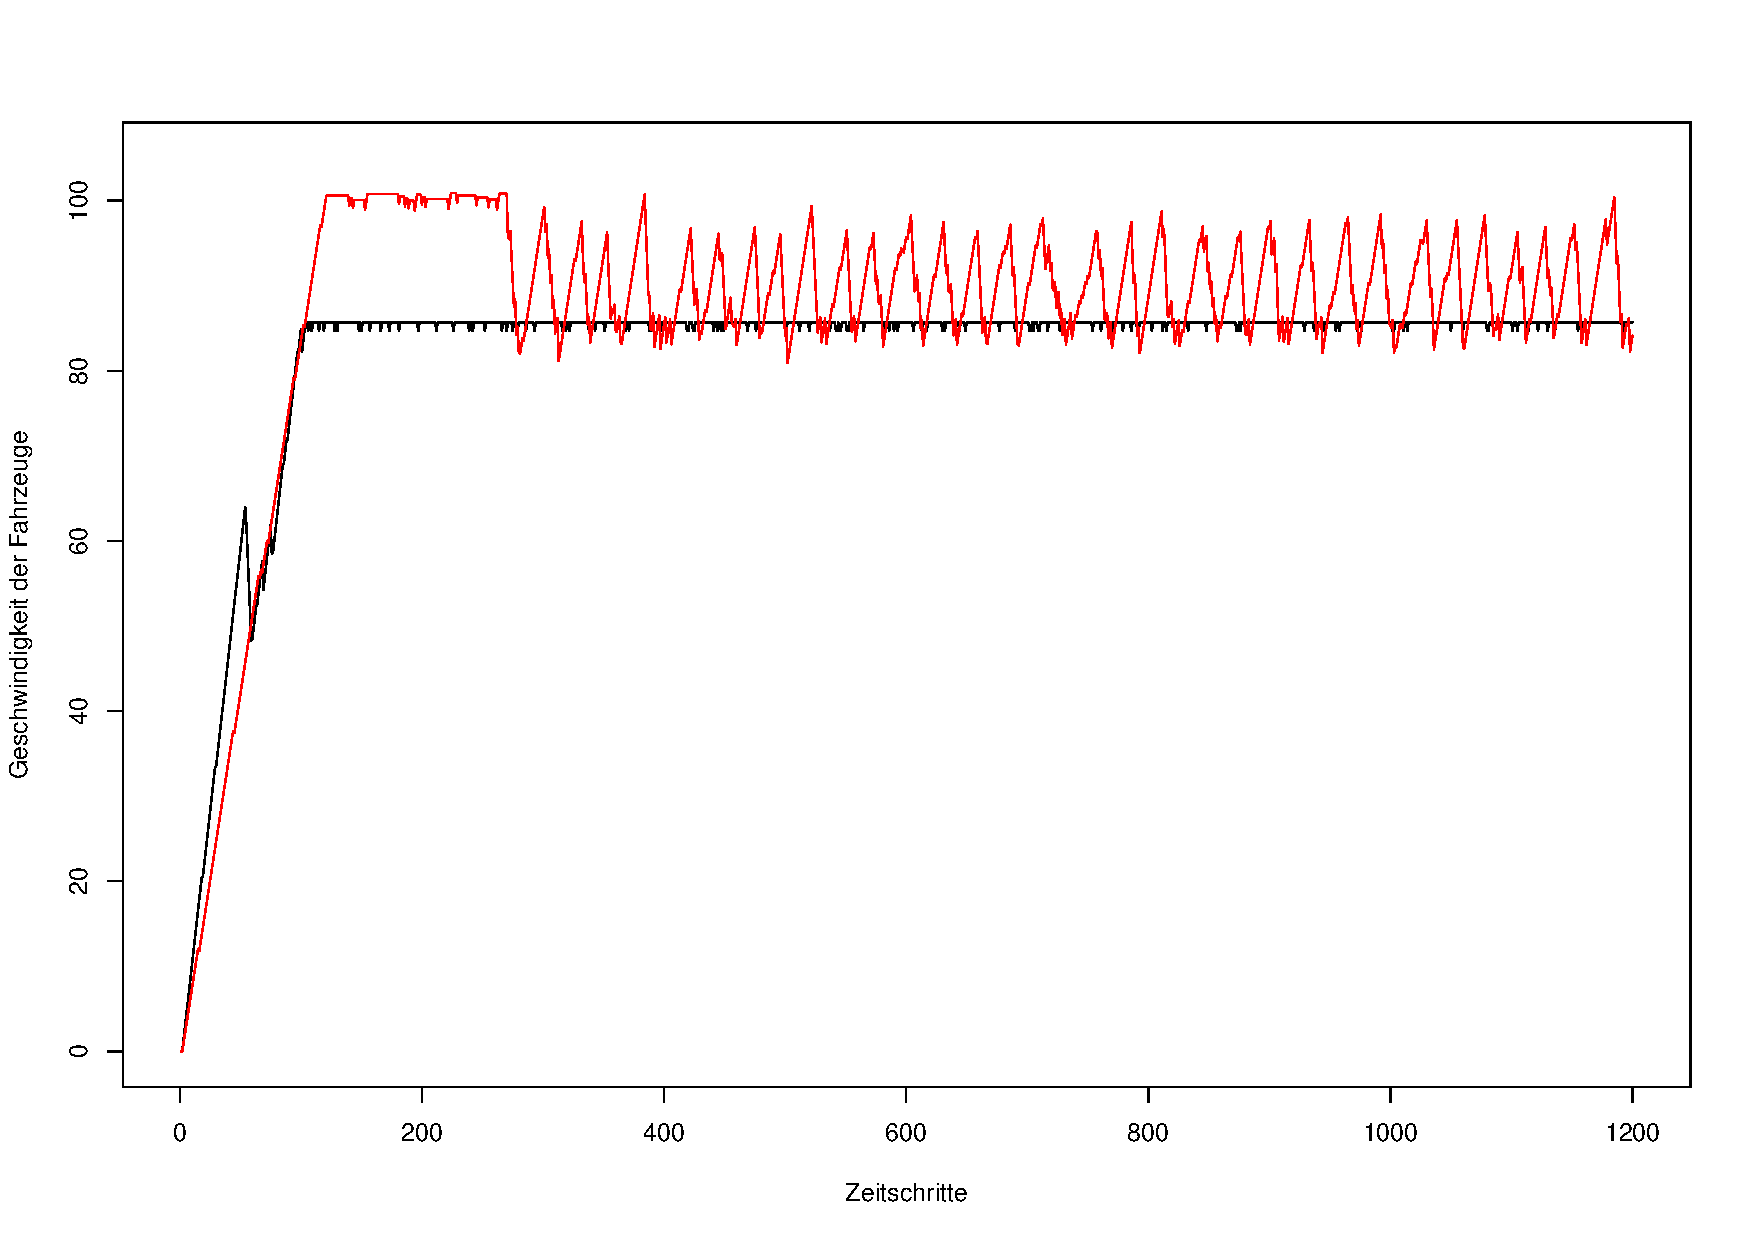
\includegraphics[width=0.3\textwidth]{speed_run18}}\qquad 
   \subfigure[3. Durchgang]{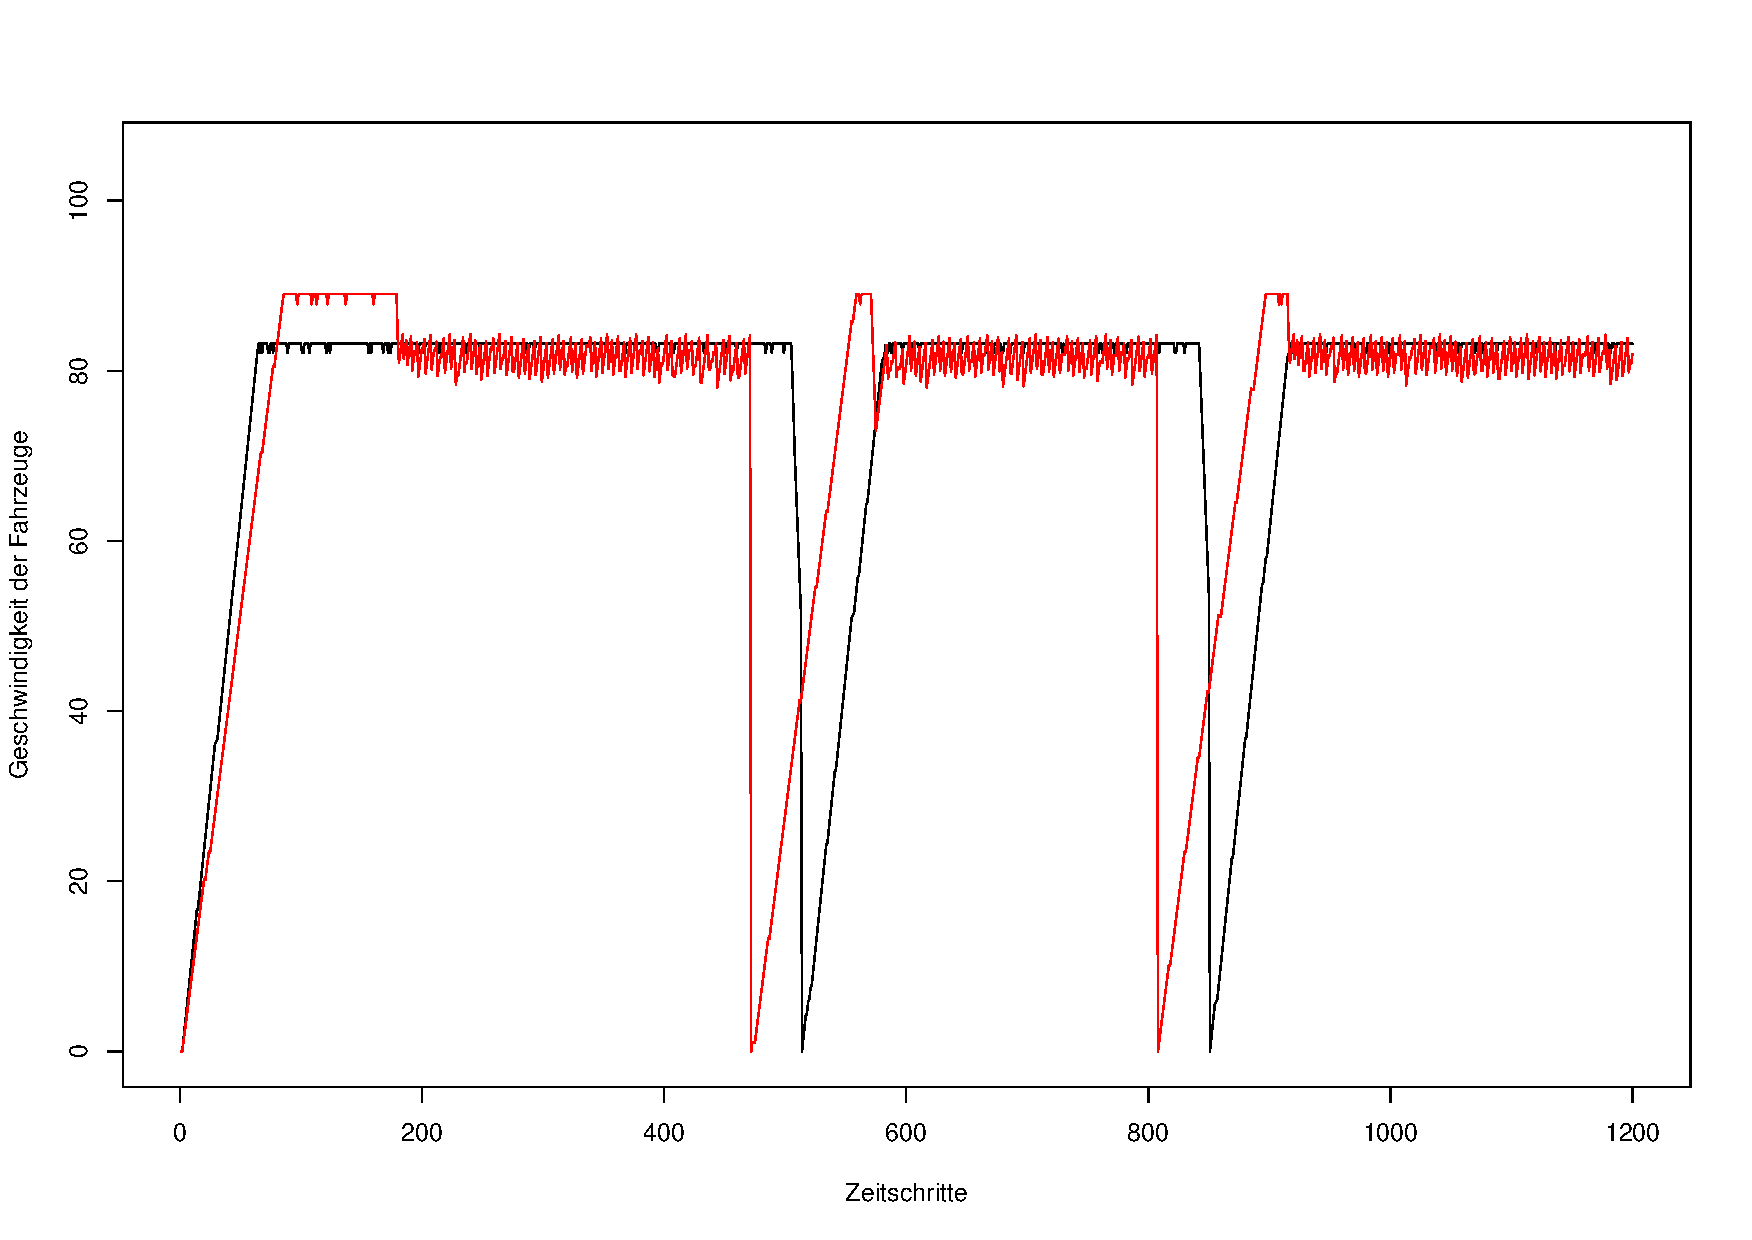
\includegraphics[width=0.3\textwidth]{speed_run19}}
  \caption{Simulationen mit Zellgröße 5,0 m und Zeitschrittlänge 0,025 min} 
  \label{figure:run17-19}
\end{figure}





\subsection{Entwicklung/Entscheidung - Festlegen der Trödelparameter}
\label{sec:lingersweetspot}

Im Originalmodell wird dem jeweiligen Fahrzeug im Trödelfall eine Geschwindigkeitseinheit wieder abgezogen. 
In jenem Zeitschritt erfolgt somit keine Beschleunigung, bzw. bei Fahren mit max. möglicher Geschwindigkeit wird diese reduziert. 
Auf das Abbremsen vor einem Hindernis hat dies keinen merklichen Einfluss, weil die mögliche Geschwindigkeit an Größe der vorhandenen Lücke angepasst wird.

Für die Simulation musste ein Wert gefunden werden, der dieses Verhalten annähernd trifft.
Im Laufe mehrerer Testdurchgänge schien eine Intensität der Verzögerung von $0,3$ die getätigte Beschleunigung am besten zu egalisieren. 
Hierbei ist noch die Streuung der Beschleunigungs- und Verzögerungswerte zu beachten, sodass das Trödeln unterschiedliche Effekte haben kann.

Für das Abbremsen in der Agentensimulation kann sich das Trödeln positiv auf den Bremsweg auswirken.



\subsection{Entwicklung/Entscheidung - Festlegen der view range}

Das originale Modell von Nagel und Schreckenberg legt Beschleunigung, Verzögerung und Sichtfeld sehr einfach fest.
Bedingt durch die Zellgröße von 7,5 m, die Ganzzahligkeit der Geschwindigkeit und die Zeitschrittlänge von 1 Sekunde ergeben sich Beschleunigungswerte von $7,5 \frac{m}{s^{2}}$. 
Durch die Möglichkeit, die Geschwindigkeit innerhalb eines einzigen Zeitschrittes von der Maximalgeschwindigkeit \enquote{5} auf Null zu verringern, ergibt sich theoretisch eine Verzögerung von $37,5 \frac{m}{s^{2}}$.

Die Simulationsumgebung arbeitet hier mit realen Werten zwischen $3,5$ und $7 \frac{m}{s^{2}}$ für die Beschleunigung und zwischen $8$ und $10 \frac{m}{s^{2}}$ für die Verzögerung.
Der Wert wird für jedes Fahrzeug bei der Initialisierung im Rahmen dieser Intervalle zufällig festgelegt.
Die Dosierung der möglichen Beschleunigung bzw. Verzögerung wird im Agentenscript festgelegt.

Für die Sichtweite ergibt sich für im NaSch-Modell der theoretische Wert von $5 \times 7,5 m$, also $37,5$ Meter.
Für die in der Agentensimulation vorliegenden \enquote{realen} Bremsvorgänge ist diese Entfernung unzureichend. 
Die Sichtweite im Straßenverkehr kann laut \cite{sichtweite} aufgrund von physiologischen und psychologischen Gründen in drei Zonen eingeteilt werden - \enquote{Fernorientierung/Information} auf Autobahnen etwa zwischen 600 und 360 Metern, \enquote{Bereitschaft/Entscheidung} etwa zwischen 360 und 110 Metern und \enquote{Nahorientierung/Handlung} unter 110 Metern.

Durch die fehlende Reaktionsträgheit, die maßgeblich durch die menschliche Komponente auftritt, hier aber fehlt, muss nicht die Phase der Fernorientierung ausgeschöpft werden. 
Ein Wert der Sichtweite mittig im Intervall der Entscheidung genügt, um bis zum Beginn der Handlungsphase \enquote{tätig zu werden}.

Für die Sichtweite wurde der Wert 250 m gewählt.
Dieser liegt ungefähr mittig im Intervall und gibt den Agenten genügend Raum für Reaktionen. 
In den Agentenplänen wird schließlich die Handlung durch Bedingungen auf einen Bereich unter 110 m beschränkt.



\subsection{Problem - Sichtfeld der Fahrzeuge}

Um die Position eines anderen Fahrzeugs in der Umwelt festzustellen, kann die Richtung, in der dieses sich befindet, bestimmt werden.
Die Simulationsumgebung hatte für das Sichtfeld der Fahrzeuge eine Unterteilung in acht Sektoren vorgesehen, so dass neben den Richtungen vorwärts, rückwärts, links und rechts auch Unterscheidung in Zwischenschritte links vorwärts, rechts vorwärts usw. möglich war, siehe \cref{figure:car-view-sectors}(a).

\begin{figure}[hptb]
  \centering 
   \subfigure[acht Sektoren]{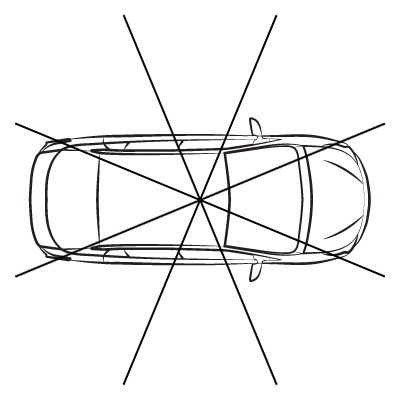
\includegraphics[width=0.3\textwidth]{car-view-8sectors}}\qquad 
   \subfigure[zwei Sektoren]{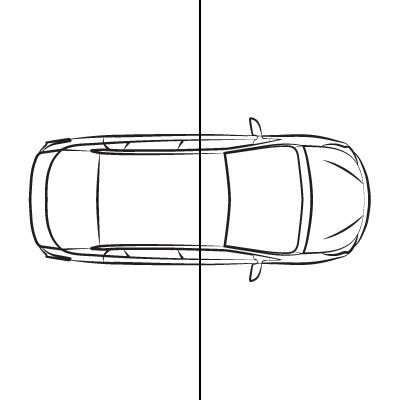
\includegraphics[width=0.3\textwidth]{car-view-2sectors}}\qquad 
   \subfigure[vier Sektoren]{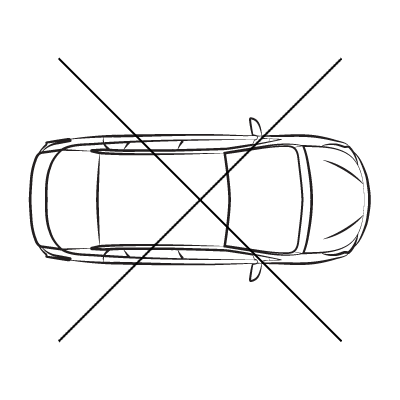
\includegraphics[width=0.3\textwidth]{car-view-4sectors}}
  \caption{mögliche Sichtfelder eines Fahrzeugs, Quelle: Auto-Silhouette vecteezy.com} 
  \label{figure:car-view-sectors}
\end{figure}

Eine solch feine Unterscheidung war nicht nötig.
Es sollte genügen, feststellen zu können, ob sich ein anderes Fahrzeug relativ zu \enquote{Ego} im vorwärtigen oder rückwärtigen Raum befindet. 
Die Abdeckung sollte ohne Unterbrechung sein.
Für die Simulation nach dem Einspurmodell von Nagel-Schreckenberg funktionierte dies ohne Probleme.

Bei einem Testlauf des Mehrspurmodells mit vier Fahrzeugen kam es zur Kollision zweier Fahrzeuge. 
Bei der anschließenden Kontrolle wurde festgestellt, dass ein Fahrzeug (vehicle0), welches sich auf der Überholspur (lane 2) befand, ein anderes Fahrzeug (vehicle20) direkt neben sich nicht \enquote*{gesehen hatte}. 
Erkennbar in der Zeile \enquote{PIA1}, die nur ausgelöst wird, wenn sich keinerlei Verkehr im Sichtfeld des Fahrzeuges befindet.
Daraufhin, so wie es der Plan vorsah, wurde zum nächsten Schritt (366) in die Hauptspur gewechselt. 
Im diesem Zeitschritt kam es dann zur Kollision.

\footnotesize\begin{verbatim}
--- step 365 ----------------
         vehicle20   in lane   1   in cell   333.0   @   74.21582362319865   kph
         vehicle2   in lane   1   in cell   282.0   @   129.99324819683062   kph
         vehicle0   in lane   2   in cell   333.0   @   99.94723620551235   kph
PIA1     vehicle0   sees no traffic at all -> Pull-in
         vehicle1   in lane   1   in cell   90.0   @   130.8321253026147   kph
--- step 366 ----------------
         vehicle20   in lane   1   in cell   4.0   @   74.21582362319865   kph
         vehicle2   in lane   1   in cell   289.0   @   131.11124225593747   kph
         vehicle0   in lane   1   in cell   3.0   @   100.80986539456516   kph
TFC100   vehicle0   has vehicle in-front of -> decelerate
COS      vehicle0   STOPPED -> collision
OUT      vehicle0   -> Pull-out attempt successful
         vehicle1   in lane   1   in cell   97.0   @   130.64144521630223   kph
\end{verbatim}
\normalsize

Das Sichtfeld der Fahrzeuge wurde zu einem Vier-Sektoren-Modell abgewandelt, siehe \cref{figure:car-view-sectors}(c), und die Pläne für Ein- und Ausscheren, der hiervon gleichermaßen betroffen sein dürfte, angepasst.
Es werden nun jeweils die beiden Sektoren kontrolliert, die die Bewegungs- bzw. Orientierungsrichtung darstellen. 
Nach vorn und hinten wird jeweils auch auf Entfernungen geprüft, seitlich auf reine Präsenz/Nichtpräsenz von anderen Fahrzeugen.

Im Rahmen dieser Umstellung wurde festgestellt, dass es bei der Richtungsbestimmung einen Fehler im Framework gab.
Die Berechnung lieferte für beide seitlichen Richtungen ein und denselben Wert.



\subsection{Problem - Simulation der Ringform der Strecke}

Die Simulation der Unendlichkeit der Strecke stellte ein Schwierigkeit für die Berechnung der Abstände zwischen Fahrzeugen dar, die sich im Sichtfeld des anderen befanden.
Es musste ein Weg gefunden werden, wie sich die Strecke virtuell um das Sichtfeld eines Fahrzeuges verlängert und dort den Verkehr vom jeweils anderen Ende der Strecke abbildet.

Zu allererst ergab sich aber das Problem, dass in der Simulation Fahrzeuge, die sich folgten, sich nicht mehr sahen, sobald das vorausfahrende den hinteren Teil der Strecke verlassen und vorn wieder eingesetzt wurde.
Nachfolgend dargestellt anhand einer Simulation mit zwei Fahrzeugen.
\enquote{...} bezeichnet Kürzungen der Ausgabe.

In Zeitschritt 315 war Fahrzeug vehicle20 gerade noch in der letzten Zelle der Fahrbahn und überschreitet diese Grenze einen Zeitschritt später.
Die Beliefliste beider Fahrzeuge ist ab dem Schritt 316 leer.
Erst nach vier Zeitschritten hat auch das Folgefahrzeug (vehicle0) die Grenze überschritten und ist ab Zeitschritt 320 wieder für Fahrzeug 20 sichtbar (andersherum ebenso).

\footnotesize\begin{verbatim}
----- step 315 ----------------
      vehicle0   -> BELIEFLIST   [view/vehicle[id[vehicle20], ... direction[forward[]]]]]]
      vehicle20   -> BELIEFLIST   [view/vehicle[id[vehicle0], ... direction[backward[]]]]]]
      vehicle0   in lane   1   in cell   331.0   @   87.11188616490347   kph
      vehicle20   in lane   1   in cell   400.0   @   88.65039571533352   kph
----- step 316 ----------------
      vehicle0   -> BELIEFLIST   []
      vehicle20   -> BELIEFLIST   []
      vehicle0   in lane   1   in cell   345.0   @   87.89778423377561   kph
      vehicle20   in lane   1   in cell   14.0   @   88.65039571533352   kph
----- step 317 ----------------
...
----- step 318 ----------------
...
----- step 319 ----------------
      vehicle0   -> BELIEFLIST   []
      vehicle20   -> BELIEFLIST   []
      vehicle0   in lane   1   in cell   387.0   @   89.01152857206483   kph
      vehicle20   in lane   1   in cell   56.0   @   88.65039571533352   kph
----- step 320 ----------------
      vehicle0   -> BELIEFLIST   [view/vehicle[id[vehicle20], ... direction[forward[]]]]]]
      vehicle20   -> BELIEFLIST   [view/vehicle[id[vehicle0], ... direction[backward[]]]]]]
      vehicle0   in lane   1   in cell   1.0   @   89.79742664093698   kph
      vehicle20   in lane 1 in cell 70.0 @ 88.65039571533352 kph
\end{verbatim}
\normalsize

Für die Simulation mit mehreren Fahrzeugen stellte dies insbesondere ein Problem dar, weil eine Stauwelle, die sich dem Anfang der Strecke näherte, von Fahrzeugen am Ende der Strecke nicht erkannt werden konnte.
Dies führte zu dem Verhalten, dass Fahrzeuge vom Ende der Strecke an den Anfang gesetzt werden sollten, dort aber nicht gesetzt werden konnten.
Die Simulationsumgebung sieht hier vor, dass das Fahrzeug auf die letzte freie Zelle hinter das jeweils letzte Fahrzeug gesetzt wird.

Es ergab sich bei den Simulationsläufen ein Häufung von Positionspunkten im negativen Teil der Strecke. 
Als Beispiel siehe [PLOT].

Nach der Behebung dieses Fehlers konnten dann auch Stauwellen beobachtet werden, die sich vom Streckenanfang herüber hinaus am Streckenende fortsetzten. 



\subsection{Ergänzungen/Ausblick/Erweiterungen}

Im Jahr 2015 wurde bei einer Studie der London School of Economics and Political Science (LSE) im Auftrag des Reifenherstellers Goodyear, siehe \cite{fahrer-typen}, festgestellt, dass man Autofahrer in sieben Typen einteilen kann.

\begin{itemize}
	\item the \enquote{teacher}, der Lehrer: möchte, dass andere Fahrer wissen, was sie falsch gemacht haben und erwartet Anerkennung für seine Anstrenungen andere zu belehren
	\item \enquote{the Know-it-all}, der Besserwisser: denkt, dass er von inkompetenten Schwachköpfen umgeben ist und schreit diese gelegentlich auch schon einmal an, während er sicher in seinem Auto sitzt
	\item \enquote{the Competitor}, der Wettkämpfer: muss vor allen anderen Fahrern sein und reagiert verärgert, wenn sich diesem Ziel jemand entgegen stellt, beschleunigt evtl. falls jemand zu überholen versucht oder schließt die Lücke um ein Einfädeln unmöglich zu machen
	\item \enquote{the Punisher}, der Bestrafer: möchte jeden anderen Fahrer für gefühltes Fehlverhalten bestrafen, steigt ggf. aus dem Auto aus, um andere Fahrer direkt zu konfrontieren
	\item \enquote{the Philosopher}, der Philosophische: akzeptiert Fehlverhalten problemlos und versucht dieses rational zu erklären, versteht es seine Gefühle im Auto zu kontrollieren
	\item \enquote{the Avoider}, der Vermeider: behandelt Fahrer, die sich daneben benehmen, unpersönlich, tut sie als Gefahr ab
	\item \enquote{the Escapee}, der Flüchter: hört Musik oder spricht am Telefon, um sich zu isolieren, lenken sich mit ausgewählten sozialen Beziehungen ab, um nicht mit anderen Fahrern auf der Straße beschäftigen zu müssen, in erster Linie ist es aber eine Strategie, das Aufkommen von Frust zu vermeiden
\end{itemize}

Für zukünftige Entwicklungen der Simulation könnte man für diese oder ähnliche Fahrertypen Profile ausarbeiten und anlegen, die sich auf Abstands-, Beschleunigungs- und Verzögerungsverhalten auswirken.
So könnte noch eine weitere Komponente mit Hinsicht auf Realitätsnähe geschaffen werden. 